%\section{Exploração do Dataset}
%
%Numa primeira fase foram criadas funções para explorar o conjunto de dados. \\
%
%A função \textbf{col\_names} retorna-nos uma dataframe com todos os nomes das colunas. A função \textbf{n\_contracts} retorna-nos o número de linhas, ou seja, o número de contratos totais, da base de dados. \\
%
%Foi desenvolvida, também, uma função \textbf{h} que permite ver uma dataframe de forma mais apresentável.\\
%
%\textit{É preciso criar uma função com o código que já tenho para categorizar os contratos de acordo com o tipo de procedimento. Idem para o tipo de contrato.} \\

 

%\begin{table}[H]
%	\centering
%	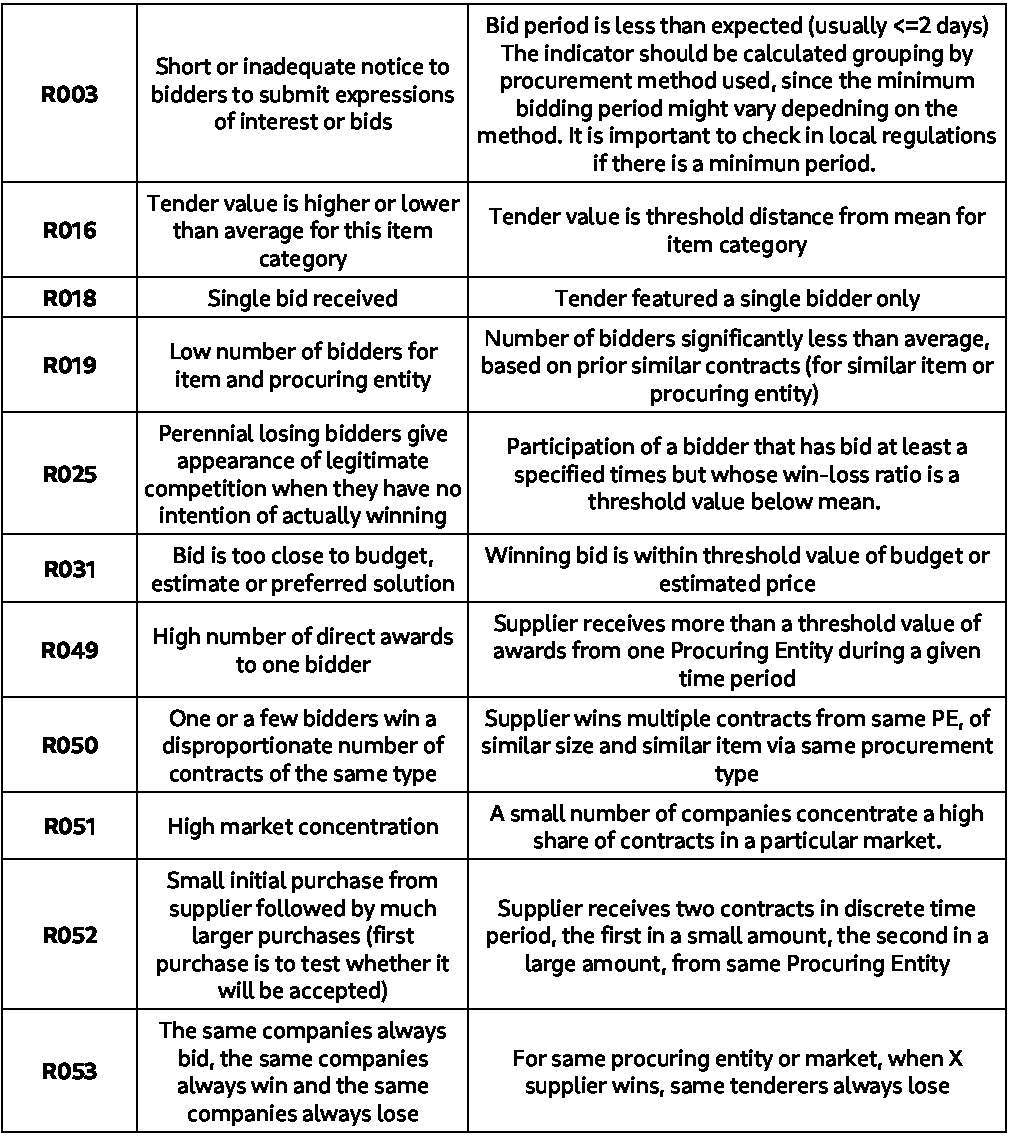
\includegraphics[width= \textwidth]{tabelas/tabela_rf.pdf}
%	\caption{}
%	\label{}
%\end{table}



 

%\section{Funções Auxiliares}
%
%Para a construção das \textit{flags} são necessárias outras funções mais simples. Certas funções irão ter um único propósito e os outputs de certas funções irão ser usados como inputs de outras funções. \\
%
%Para identificar um contrato necessitamos do seu id. Assim, criou-se uma função \textbf{all\_ids} que retorna os ids de todos os contratos da base de dados. Contudo, como não vamos trabalhar com todos os tipos de contratos e procedimentos, é necessário filtrar estes ids.
%Para tal, criaram-se as funções \textbf{ajustes\_dir}, \textbf{consulta\_prev} e \textbf{concurso\_pub} que retornam os ids de todos os ajustes diretos, consultas prévias e concursos públicos, respetivamente. \\
%
%De seguida, filtraram-se os contratos por tipo de procedimento e por CPV. Para isso, criou-se a função \textit{cpv\_direto} que retorna todos os ids de ajustes diretos para serviços de consultoria em IT ( todos os CPV's começados por 72). De seguida, foi feito o mesmo para contratos públicos na função \textit{cpv\_cpub}. De forma a generalizar, criou-se a função \textit{cpv} que retorna todos os ids de contratos de um tipo de procedimento e para um determinado CPV. Tanto o tipo de procedimento como os primeiros 2 algarismos do CPV são parâmetros de entrada da função. \\
%
%
%Para começar, criaram-se duas funções que permitem ver qual é o contrato associado a um determinado id. A função \textit{contrato} tem como input um único id de um contrato ( todas estas funções dizem respeito à tabela \textit{contratos} da DB) e retorna uma dataframe com uma única linha referente ao contrato associado a esse mesmo id. A função \textit{contratos} faz exatamente a mesma coisa mas para um conjunto de id's. \\
%
%Quando as flags estiverem construídas e quisermos ver o anúncio de um contrato suspeito no site do basegov, podemos fazê-lo usando a função \textit{url} que, novamente, tem como parâmetro de entrada o id de um contrato. Esta função pode ter bastante utilidade nos casos que chamam bastante a atenção, como por exemplo, quando se viu um ajuste direto de 3 milhões de euros. \\

No website da OCDS encontra-se disponível para descarregar uma folha de cálculo em Excel com 73 red flags \cite{spreadsheet1} \cite{spreadsheet}, tal como se encontra representado na Tabela \ref{table:flags}.

\begin{table}[H]
	\centering
	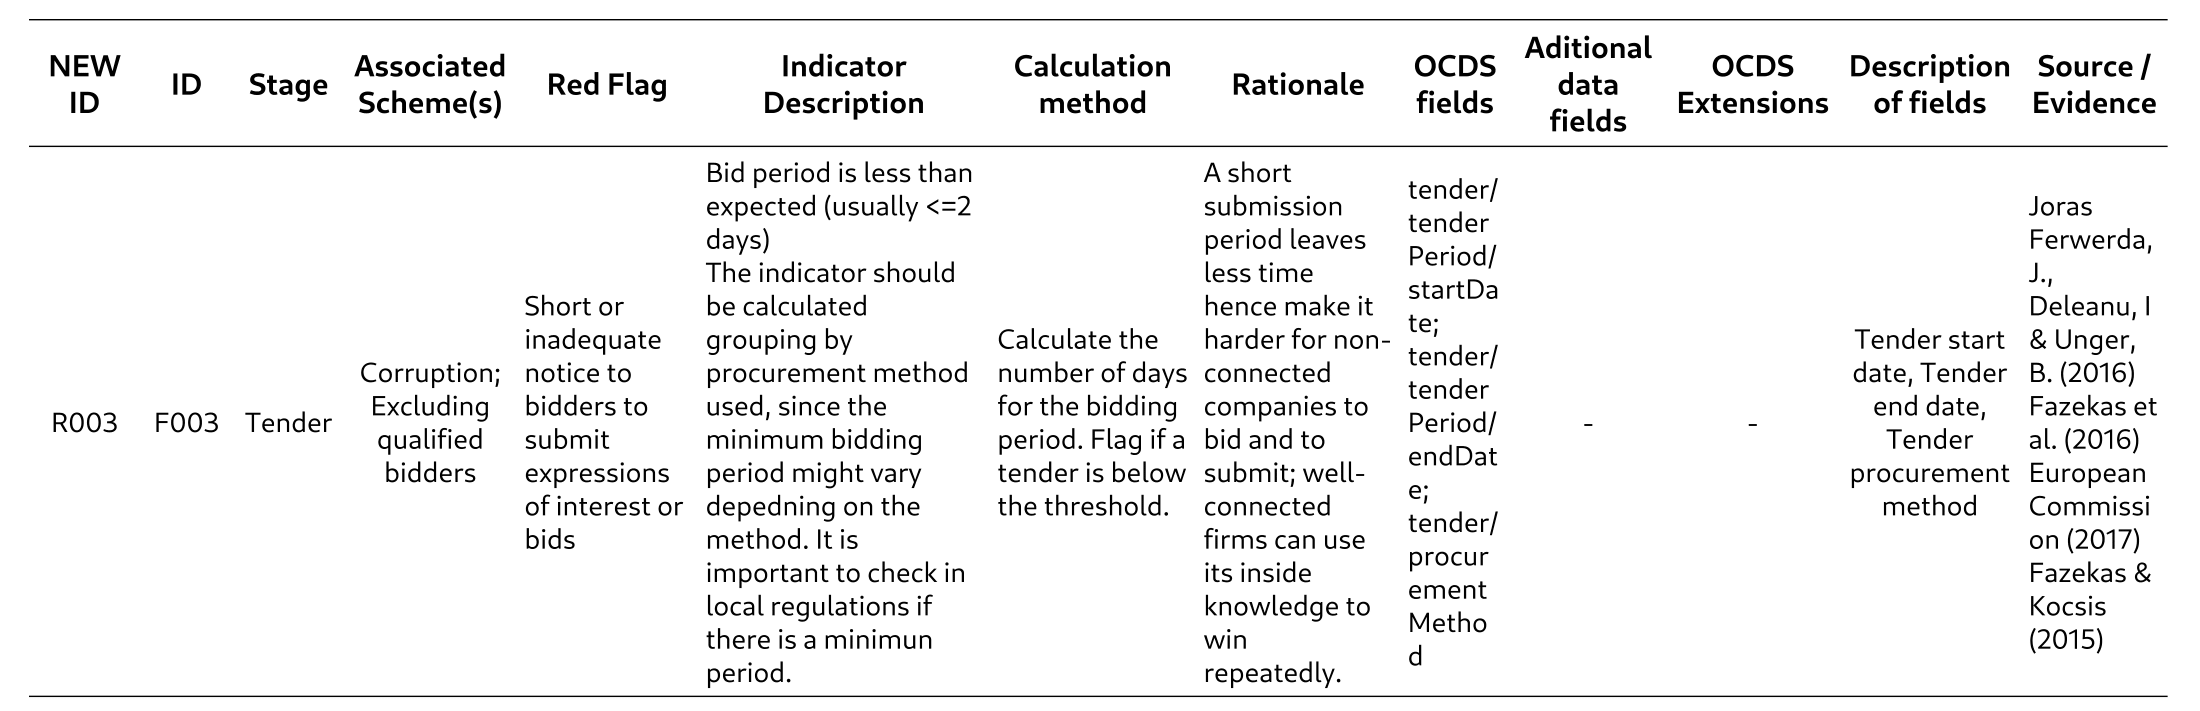
\includegraphics[width=\textwidth]{imagens/tabela_flags.png}
	\caption{Exemplo da descrição de uma flag}
	\label{table:flags}
\end{table}


A fim de construir as funções que permitam selecionar contratos anómalos, foi feita uma análise, de caráter subjetivo, relativamente ao nível de importância e de facilidade de implementação. Para cada uma das 73 flags, foi atribuído um valor de 1 a 3, tanto para o nível de facilidade de implementação como para o nível de importância. Para atribuir um valor à facilidade de implementação foi necessário ter em conta se a base de dados possuía todas as variáveis necessárias, o que nem sempre se verificou. Relativamente ao nível de importância, o critério foi mais subjetivo e serviu como uma ferramenta de filtragem. Após esta classificação, foi realizada uma média ponderada destas classificações, com uma peso atribuído de 0.6 ao primeiro parâmetro e de 0.4 ao segundo parâmetro. Dessa forma, foi possível filtrar todas as flags e excluir aquelas que não eram passíveis de implementar. 

Além destes indicadores, foram desenvolvidos outros 3, após discussão, que se acreditava terem valor para o resultado final. Estes indicadores foram construídos tendo em conta o CCP, as variáveis presentes na base de dados e flags definidas pela OCDS. 

Nas secções que se seguem, todos os indicadores establecidos pela OCDS são identificados pela letra R e um número, enquanto que aqueles que os que foram desenvolvidos em equipa são identificados por RF e um número.

Os contratos coletados encontram-se todos guardados numa tabela chamada \textit{contratos\_basegov} numa base de dados em PostgreSQL. De modo a construir os indicadores que se encontram nos capítulos seguintes, foi necessário criar quatro tabelas adicionais auxiliares:

\begin{my_itemize}
	\item concursos\_publicos: tabela para onde foram copiadas as principais variáveis referentes a concursos públicos
	
	\item ajustes\_diretos: tabela para onde foram copiadas as principais variáveis referentes a ajustes diretos em regime geral
	
	\item cpv\_stats: tabela que contém os indicadores estatísticos relativamente ao número de entidade de concorrentes por divisão de CPV. Para cada divisão de CPV, dentro de todo o conjunto de concursos públicos, foi calculado o número total de contratos celebrados (count), o número total de entidades que se candidataram a todos os concursos (nec\_t), o número médio de entidades concorrentes por concurso, desvio padrão, mínimo, máximo, Q1, Q2 e Q3. 
	
	\item preco\_stats: Esta tabela segue uma filosofia similar à apresentada anteriormente. Contudo, em vez de se fazer uma análise por divisão de CPV, esta é feita a partir do Grupo do CPV (os três primeiros dígitos) a fim de ter uma maior granularidade. 
\end{my_itemize}


Na Figura \ref{fig:basededados} encontra-se um esquema da relação entre as diferentes tabelas. Para efeitos de concisão do diagrama apenas são apresentadas algumas das principais colunas. As colunas que se encontram a vermelho, explicadas nas secções que se segue, dizem respeito a colunas auxiliares para a construção dos indicadores

\begin{figure}[H]
	\centering
	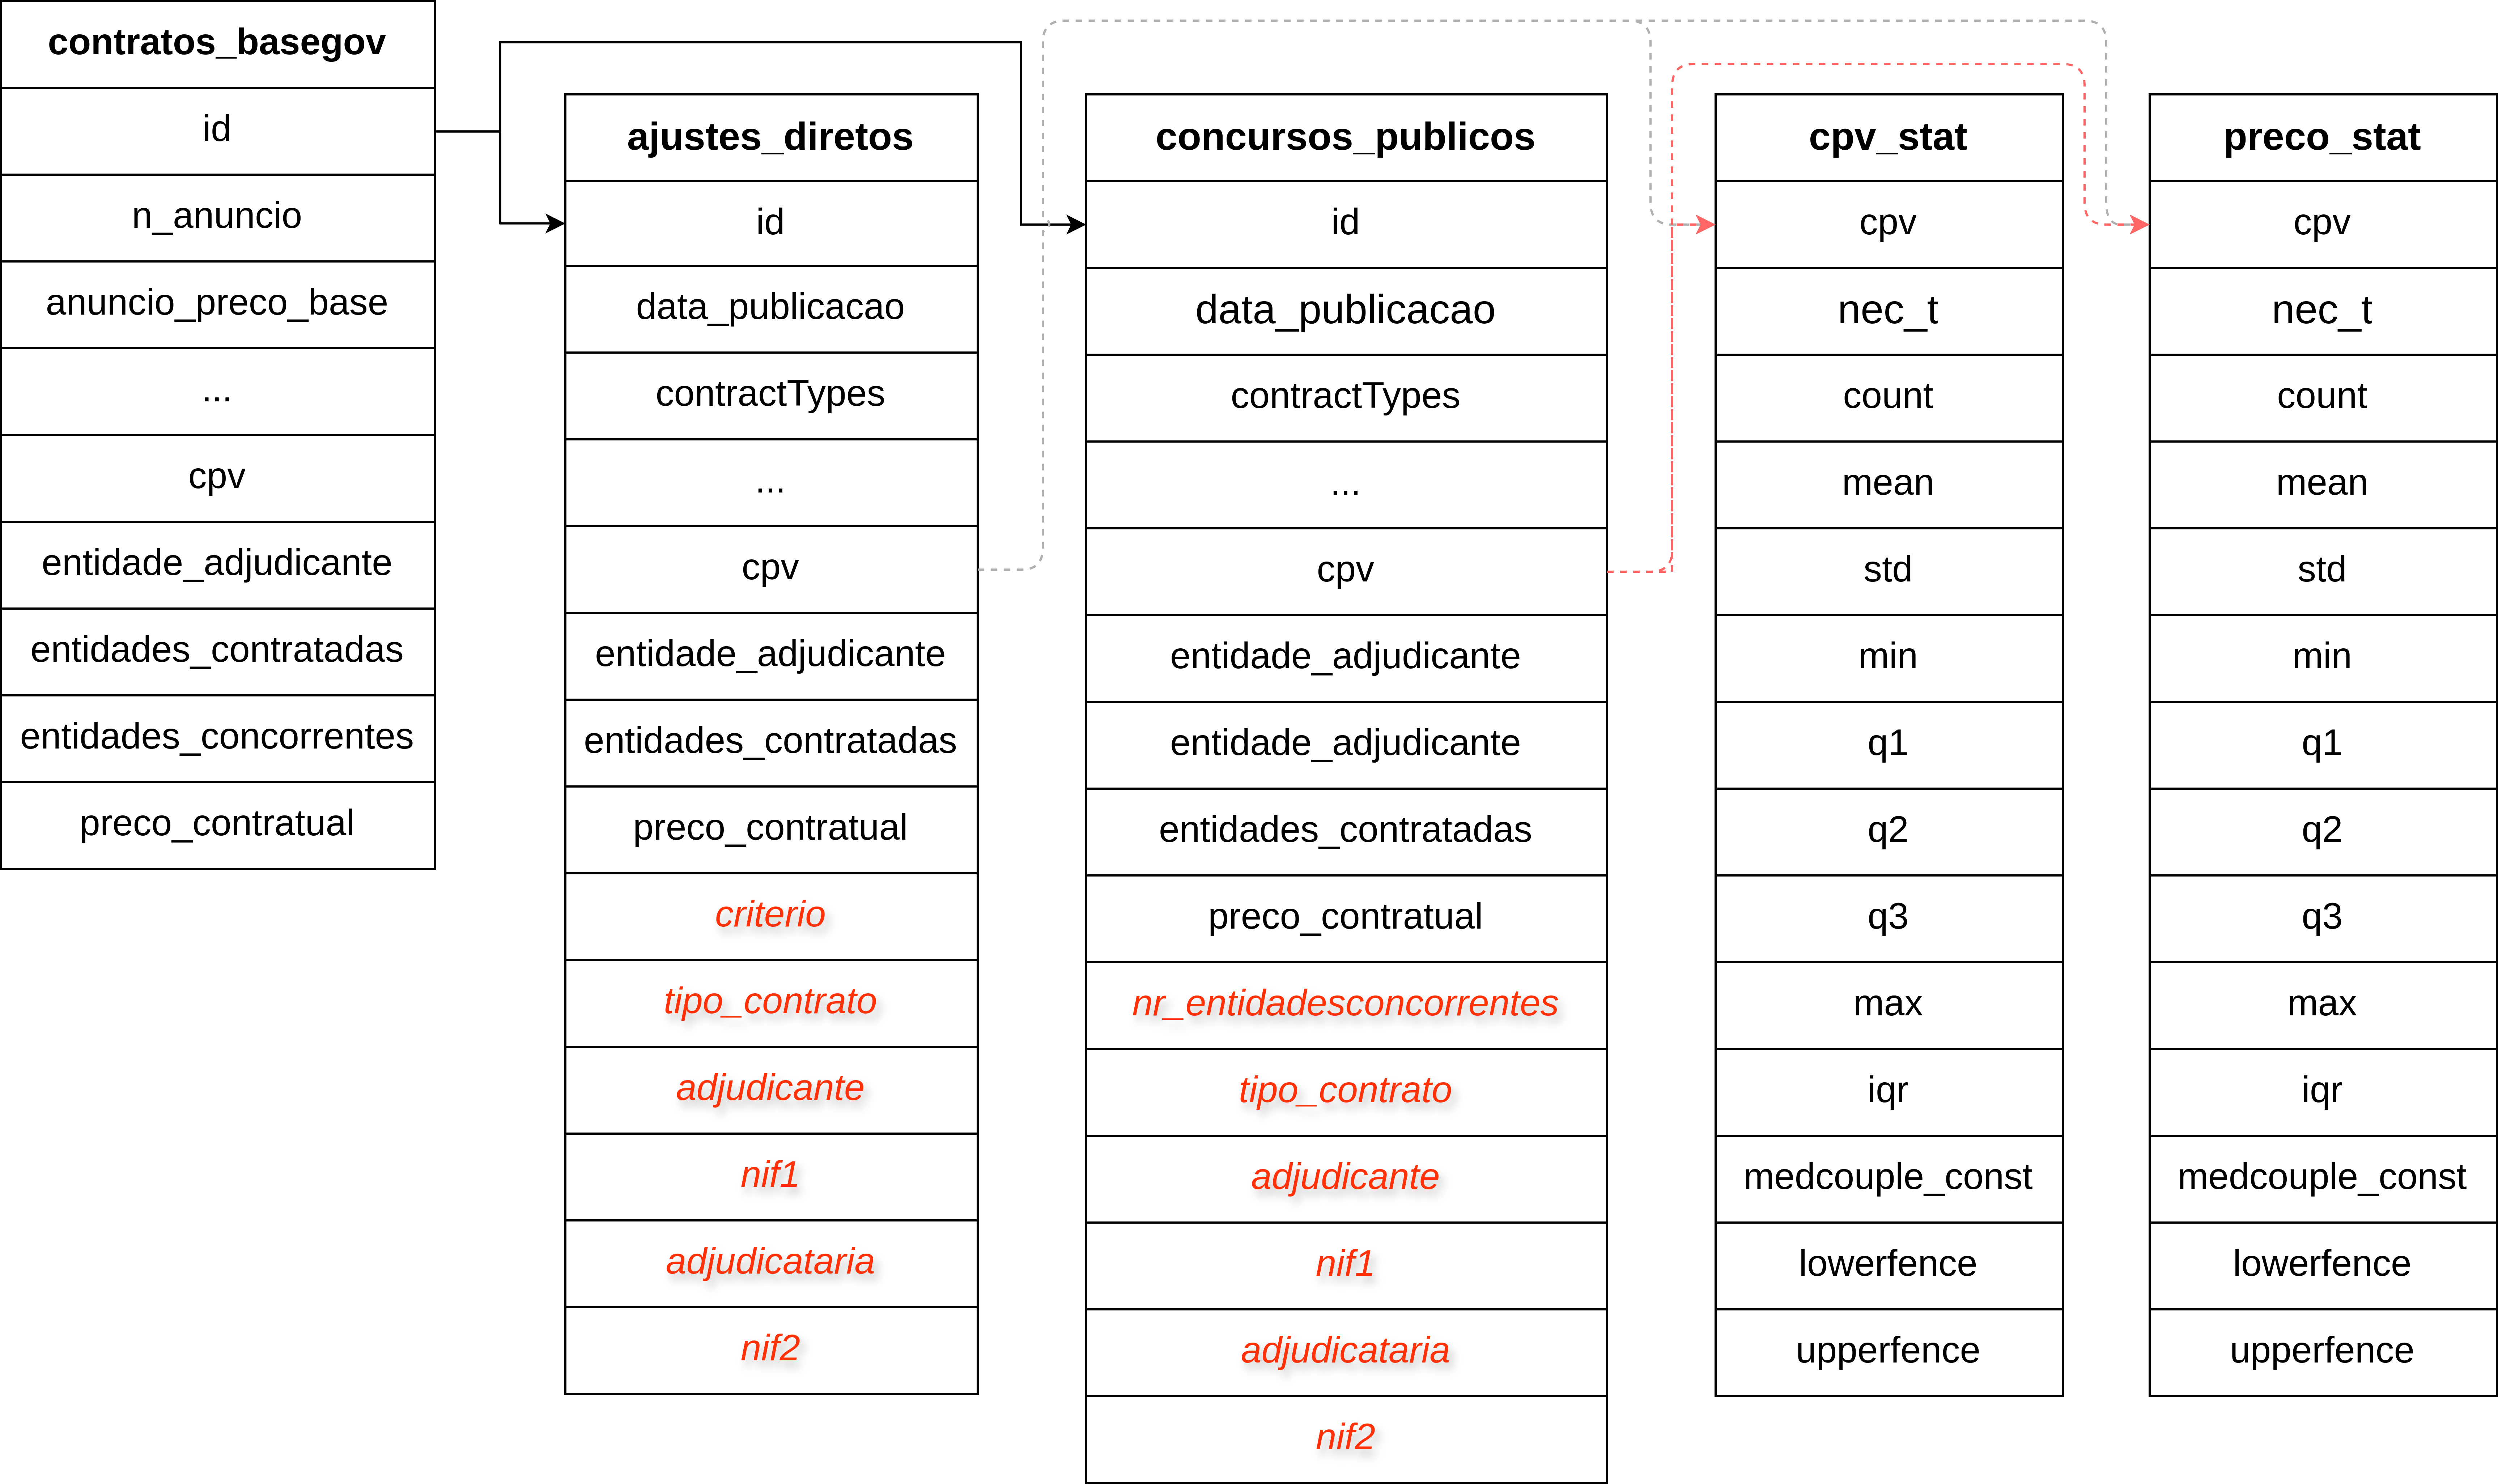
\includegraphics[width=0.9\textwidth]{imagens/basedadostabelas.png}
	\caption{Organização das tabelas da base de dados.}
	\label{fig:basededados}
\end{figure}





\section{RF1: Verificação dos Preços Contratuais para Ajustes Diretos em Regime Geral}


Como foi apresentado anteriormente na Tabela \ref{tab:4}, os ajustes diretos, consoante o tipo de obra/serviço, tem diferentes limites máximos impostos por lei relativamente ao valor de adjudicação. A fim de poder identificar os contratos que não estão em conformidade com o CCP, procedeu-se da seguinte forma. Primeiramente, criou-se uma nova tabela na base de dados, a partir da tabela original, para onde foram copiados todos os ajustes diretos em regime geral e onde foi criada um nova coluna, chamada \textbf{criterio}. De seguida, para cada um dos contratos, foi identificado o artigo utilizado para fundamentar a adoção deste tipo de procedimento, presente na coluna da fundamentação. Se o artigo pertencer entre o 17º e o 22º, é atribuído ao contrato a string \textbf{valor} na nova coluna criada. Caso contrário, é atribuído a string \textbf{material}. 

 \begin{table}[H]
 	\centering
 	\begin{tabular}{|c|c|c|c|}
 		\hline
 		\textbf{Critério}                  & \textbf{Artigos}           & \textbf{Tipo de Contrato}           & \textbf{Valor} \\ \hline
 		\multirow{3}{*}{Critério do Valor} & \multirow{3}{*}{17º a 22º} & Aquisição de bens móveis e serviços & 20000€         \\ \cline{3-4} 
 		&                            & Empreitadas de obras públicas       & 30000 €        \\ \cline{3-4} 
 		&                            & Outro tipo de contratos             & 50000 €        \\ \hline
 		Critério Material                  & 24º a 27º                  & Qualquer                            & Indefinido     \\ \hline
 	\end{tabular}
 	\caption{Valores máximos permitidos para Ajustes Diretos consoante o critério, artigo e tipo de contrato.}
 \end{table}

De seguida, foi necessário classificar os contratos relativamente à tipologia. Tal como se encontra representado na Tabela \ref{table:3}, os contratos podem ser classificados em duas grandes categorias: Bens e Serviços ou Empreitadas. Contudo, na coluna referente ao tipo de contrato não é feita esta discriminação. Assim, foi adicionada uma nova coluna a esta tabela, \textbf{tipo\_contrato}, que irá ter apenas uma das duas categorias anteriormente presentes para cada contrato. Para classificar cada contrato numa destas duas categorias fez-se uma busca da palavra \textit{obra} na string presente na coluna da tipologia de contrato. Se esta palavra estivesse contida na string, o contrato era classificado como Empreitada. Caso contrário, Bens e Serviços. 


\begin{figure}[H]
	\centering
	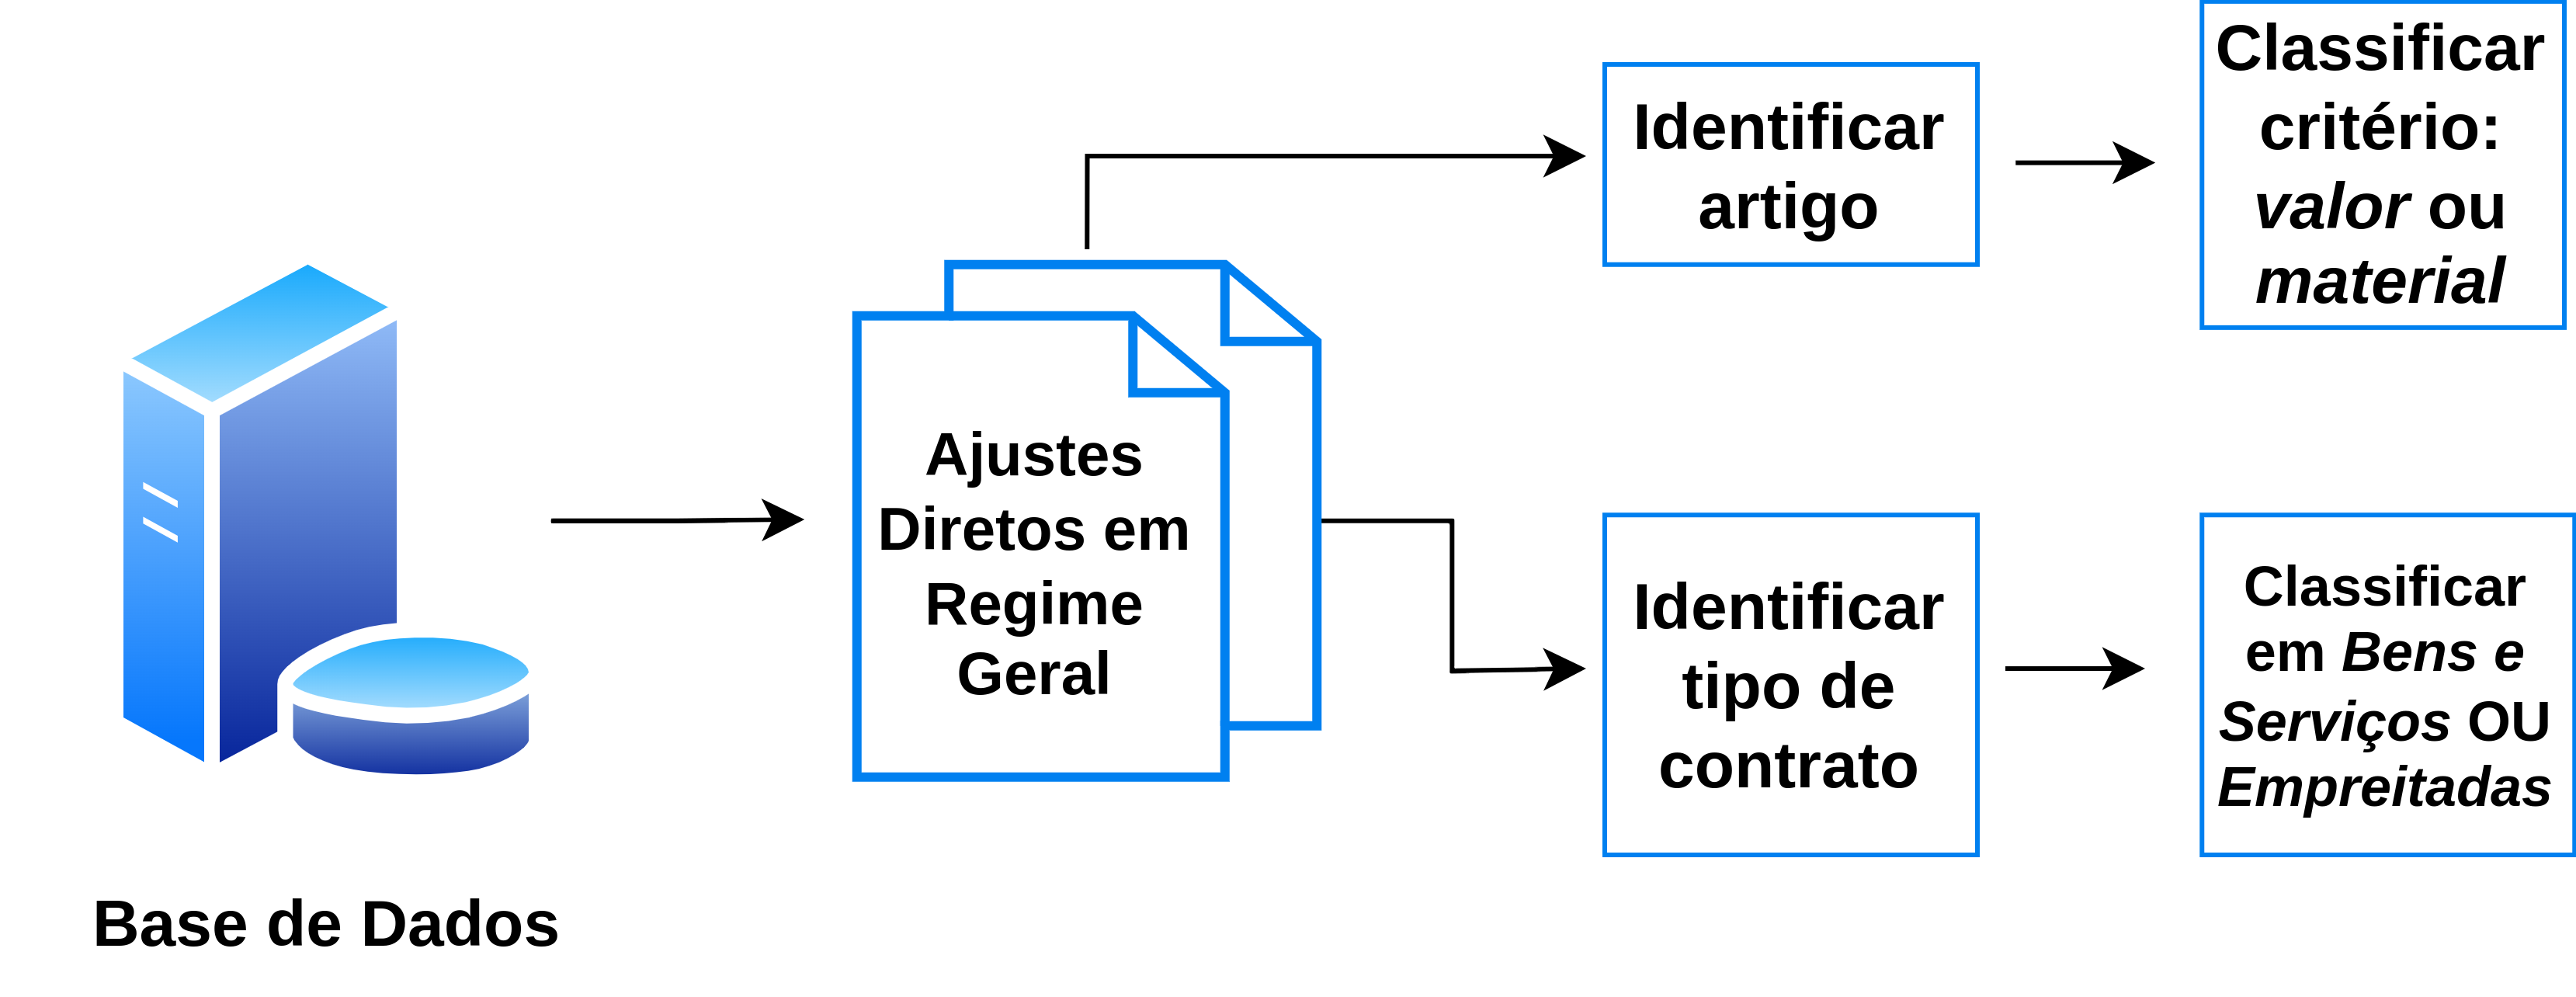
\includegraphics[width=0.9\textwidth]{imagens/rf1.png}
	\caption{Processo de classificação de ajustes diretos em regime geral}
	\label{}
\end{figure}




%\begin{lstlisting}[
%	language=SQL,
%	showspaces=false,
%	showstringspaces=false,
%	basicstyle=\ttfamily,
%	numbers=left,
%	numberstyle=\tiny,
%	commentstyle=\color{gray}, frame = single,	autogobble=true,
%	postbreak=\mbox{\textcolor{red}{$\hookrightarrow$}\space},
%	]
%	ALTER TABLE ajustesdiretos
%	ADD COLUMN artigo text;
%	
%	UPDATE ajustesdiretos
%	SET artigo = TRIM(SUBSTRING(fundamentacao 
%			FROM 1 FOR POSITION('º' IN fundamentacao)));
%\end{lstlisting}

%\begin{lstlisting}[
%	language=SQL,
%	showspaces=false,
%	showstringspaces=false,
%	basicstyle=\ttfamily,
%	numbers=left,
%	numberstyle=\tiny,
%	commentstyle=\color{gray}, frame = single,	autogobble=true,
%	postbreak=\mbox{\textcolor{red}{$\hookrightarrow$}\space},
%	]
%	ALTER TABLE ajustesdiretos
%	ADD COLUMN criterio text;
%	
%	UPDATE ajustesdiretos
%	SET criterio = CASE
%	WHEN artigo = 'Artigo 17.º' OR artigo = 'Artigo 18.º' 
%	OR artigo = 'Artigo 19.º' OR artigo = 'Artigo 20.º' 
%	OR artigo = 'Artigo 21.º' OR artigo = 'Artigo 22.º' 
%	THEN 'valor'
%	
%	ELSE 'material' 
%	END;
%\end{lstlisting}


Finda estas classificações quanto à tipologia e fundamentação, é possível identificar todos os contratos que não respeitem os valores apresentados na Tabela \ref{tab:4} a partir da seguinte \textit{query}: 

\begin{lstlisting}[
	language=SQL,
	showspaces=false,
	showstringspaces=false,
	basicstyle=\ttfamily,
	numbers=left,
	numberstyle=\tiny,
	commentstyle=\color{gray}, frame = single,	autogobble=true,
	breaklines=true,
	postbreak=\mbox{\textcolor{red}{$\hookrightarrow$}\space},
	]
	SELECT id
	FROM ajustesdiretos
	WHERE (criterio = 'valor' AND tipocontrato = 'Bens e Servicos' AND preco > 20000) OR (criterio = 'valor' AND tipocontrato = 'Empreitadas' AND preco > 30000);
\end{lstlisting}

Da totalidade de Ajustes Diretos em Regime Geral presentes na base de dados, 2.8\% (12828) destes foram adjudicados com um valor superior ao permitido por lei. Destes, 2.4\% (14812) dizem respeito a contratos de Bens e Serviços e 0.4\% (1984) a contratos de Empreitadas.


\begin{figure}[H]
	\centering
	\begin{minipage}{.45\linewidth}
		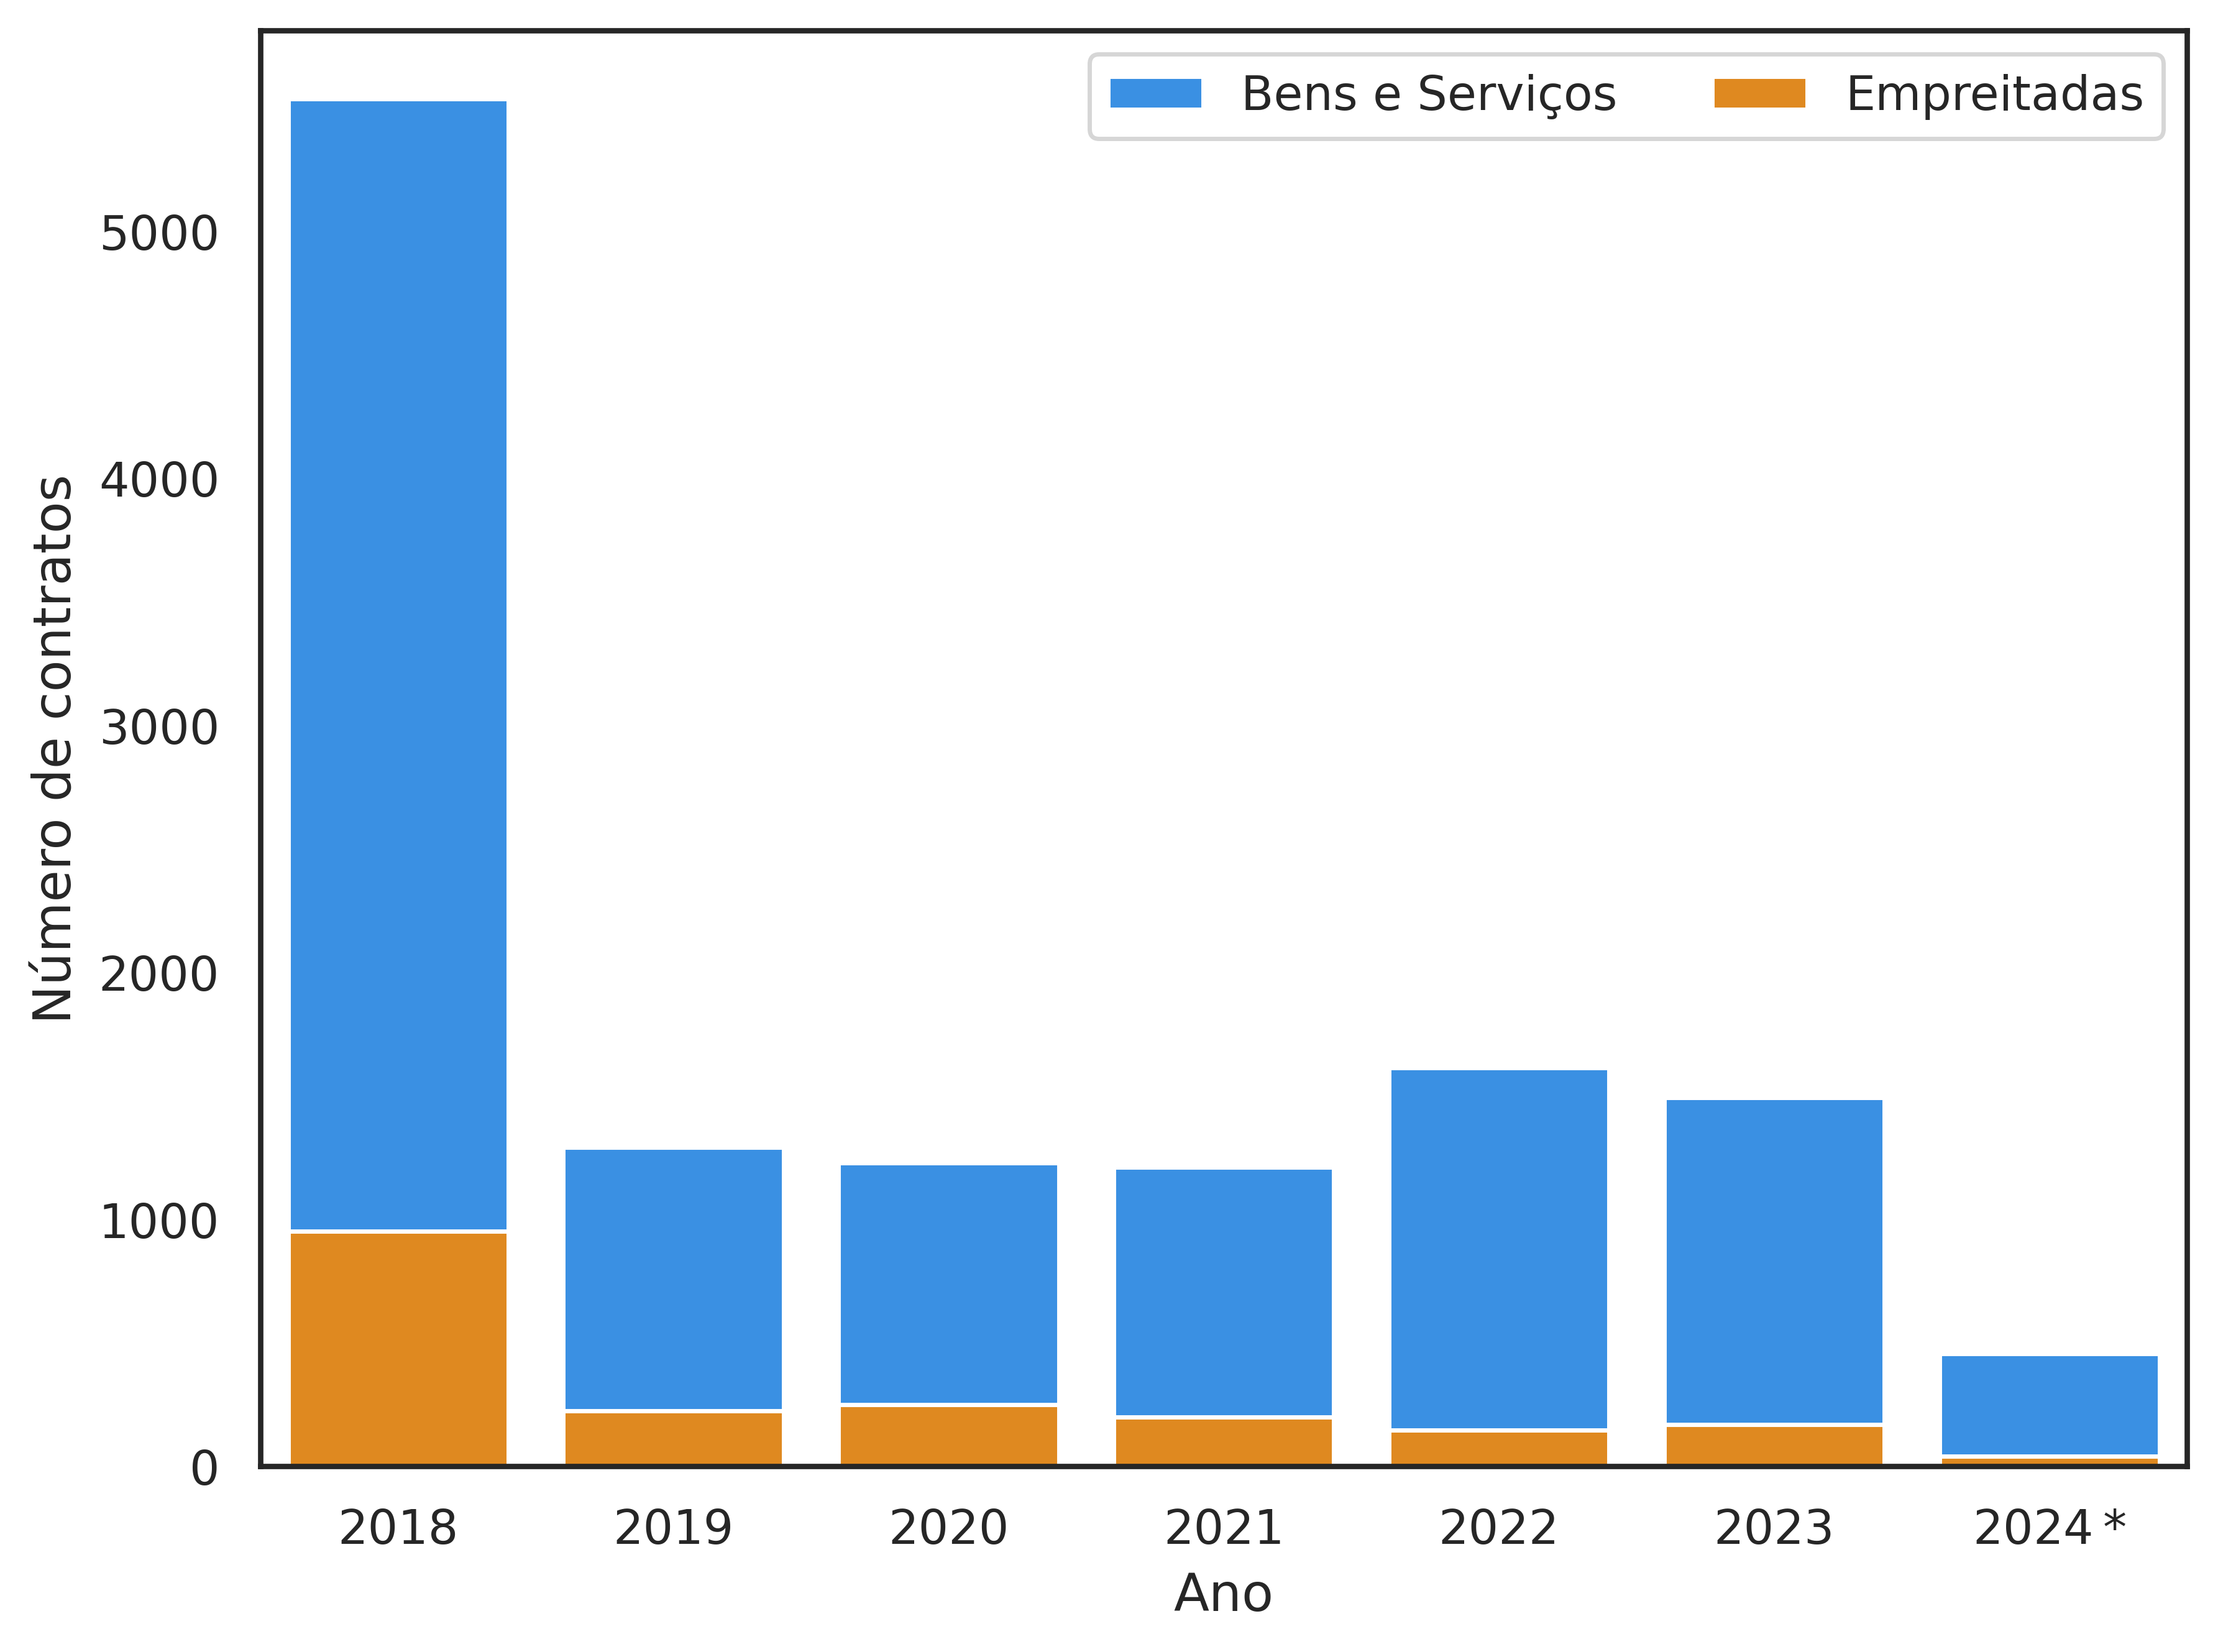
\includegraphics[width=\linewidth]{imagens/rf1/dist.png}
		\caption{Distribuição do número de contratos em inconformidade com o CCP}
		
	\end{minipage}
	\hfill
	\begin{minipage}{.5\linewidth}
		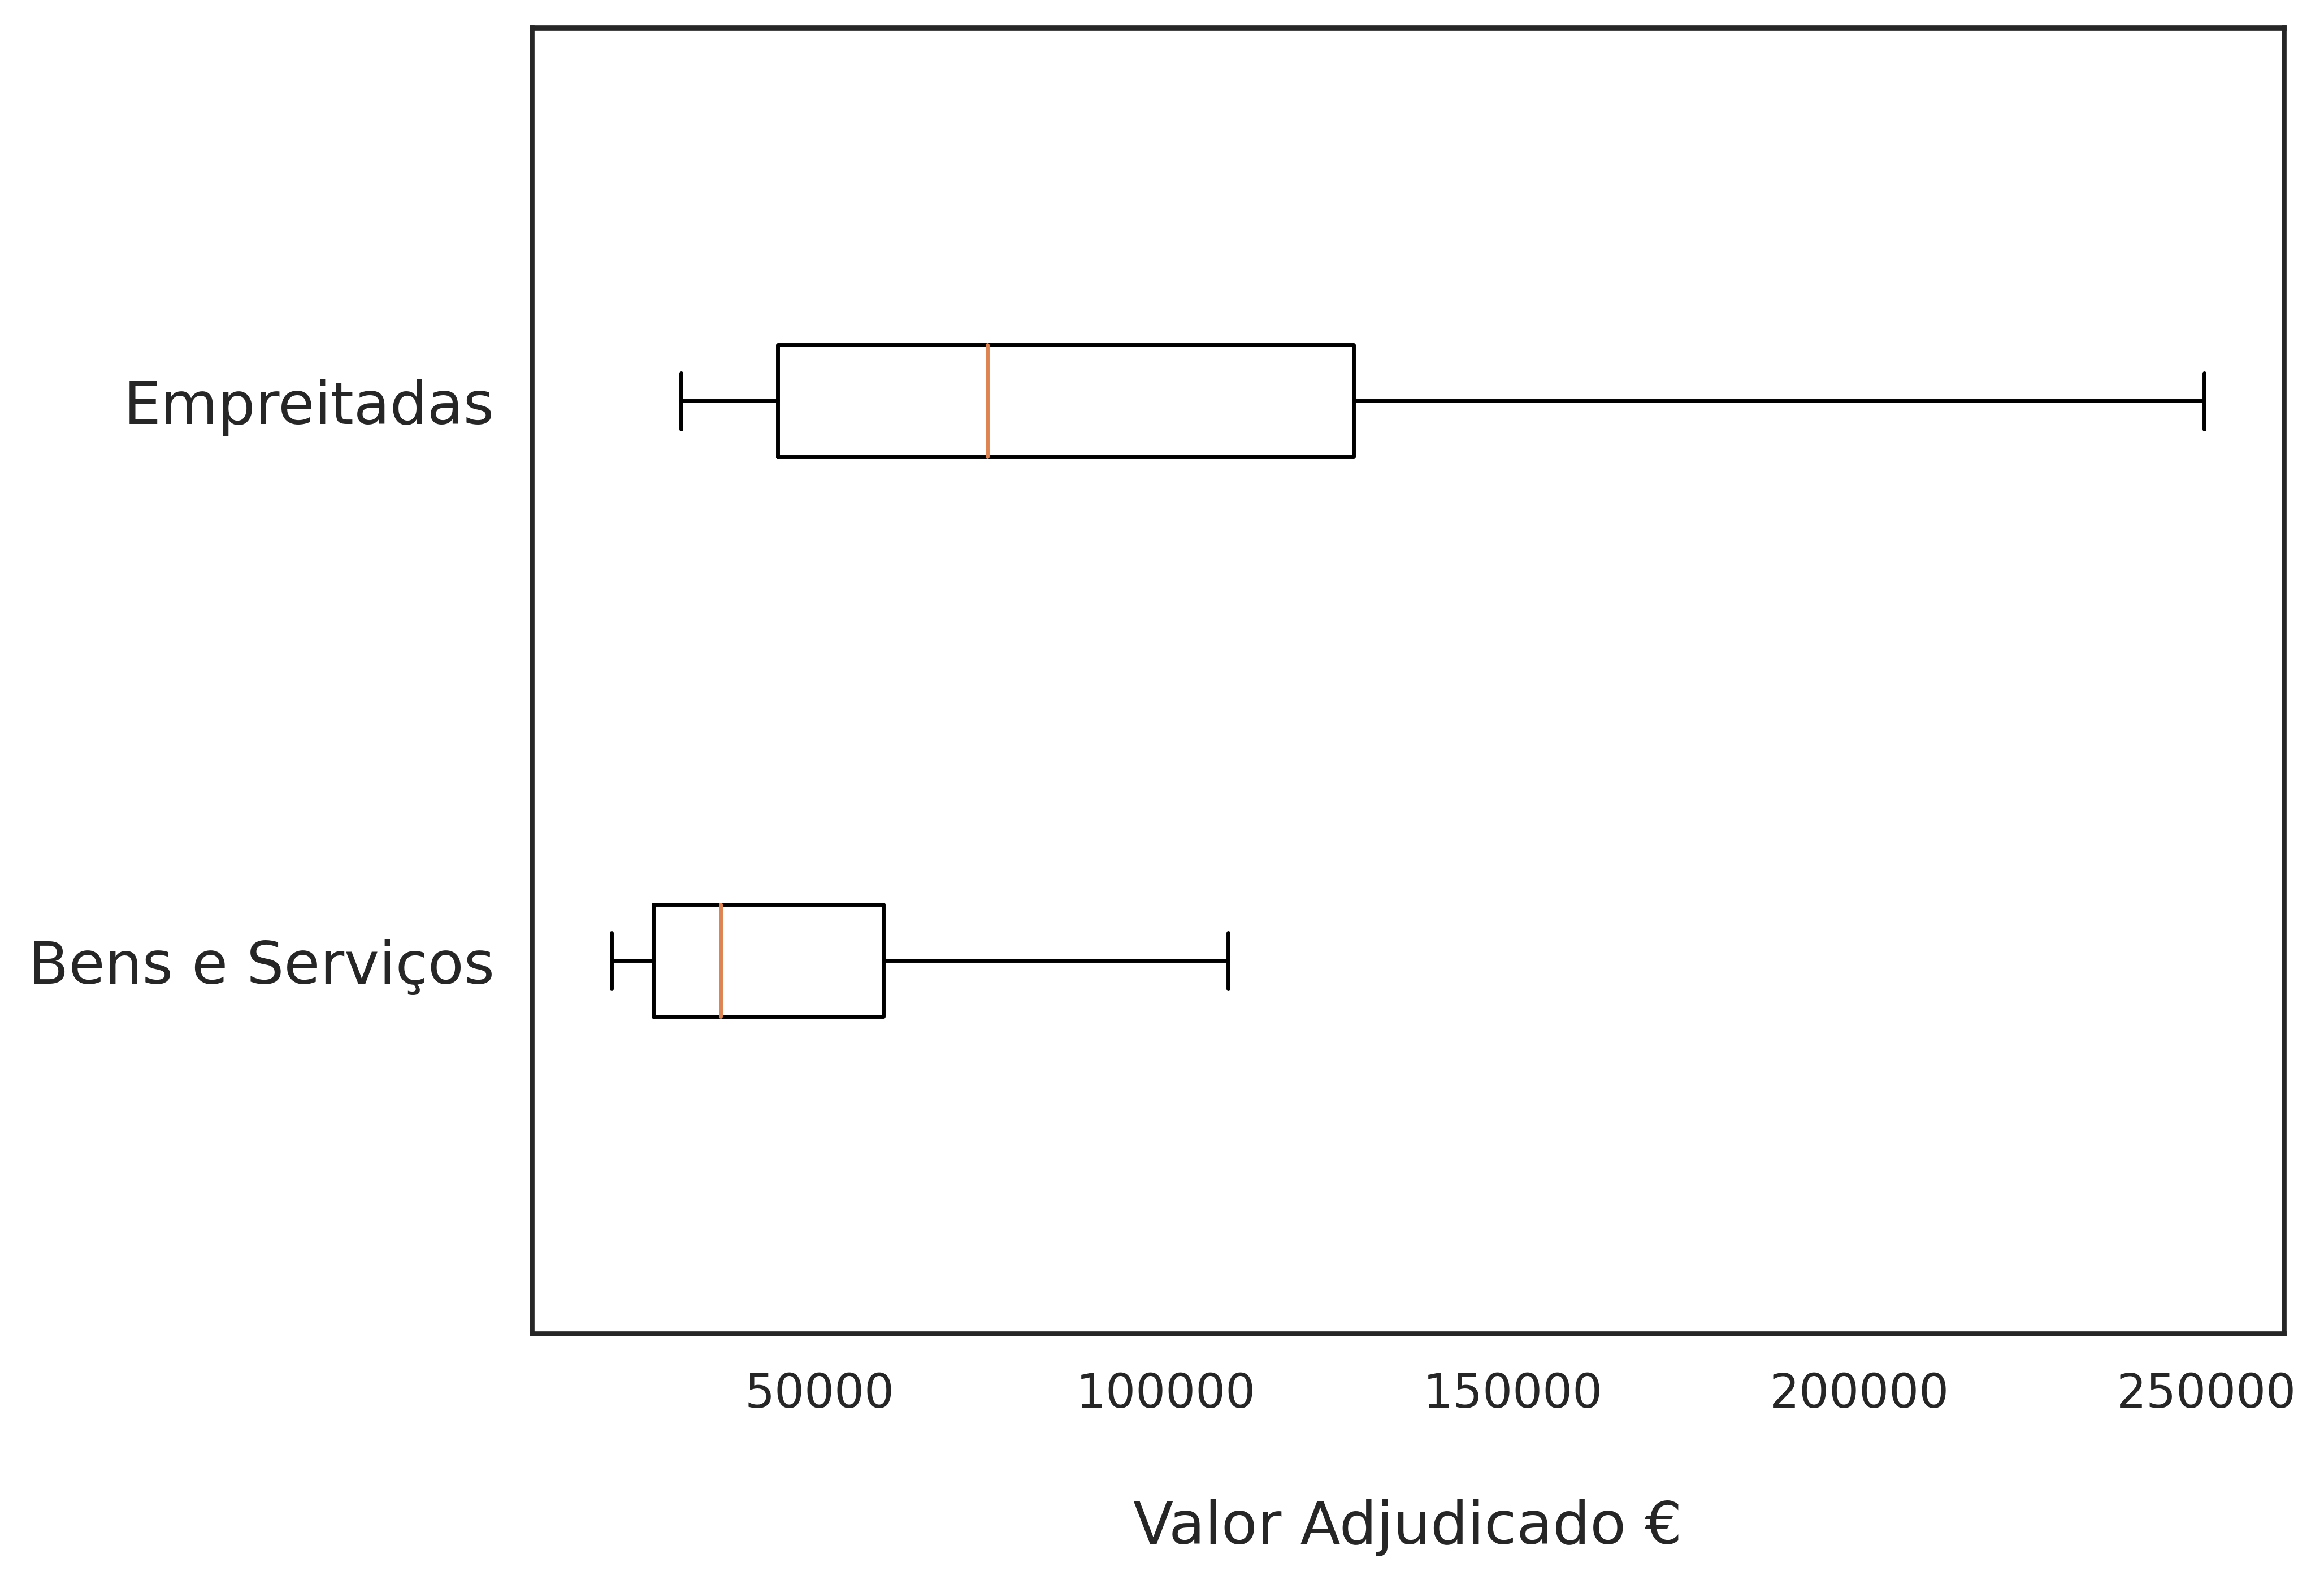
\includegraphics[width=\linewidth]{imagens/rf1/boxplot.png}
		\caption{Boxplot dos valores contratuais para os contratos em inconformidade com a lei}
		
	\end{minipage}
\end{figure}


Na Tabela \ref{tab:rf1} é possível observar quais são as entidades com o maior número de contratos celebrados em inconformidade com o CCP. 

\begin{table}[H]
	\centering
	\renewcommand{\arraystretch}{1.15}
	\setlength{\tabcolsep}{15pt}
	\resizebox{\textwidth}{!}{%
		\begin{tabular}{lc}
			\hline
			\multicolumn{1}{c}{\textbf{Entidade Adjudicante}}                                           & \textbf{Número de Contratos} \\ \hline
			Infraestruturas de Portugal, S. A.                                                          & 377                          \\
			Hospital de Santo Espírito da Ilha Terceira, E. P. E. R.                                    & 329                          \\
			Município de Ponta Delgada                                                                  & 204                          \\
			Instituto Português de Oncologia do Porto Francisco Gentil, E. P. E.                        & 203                          \\ \hline
			\multicolumn{1}{c}{\textbf{Entidade Vencedora}}                                             & \textbf{Número de Contratos} \\ \hline
			Meo - Serviços de Comunicações e Multimédia S.A                                             & 165                          \\
			Urbhorta - Construção, Gestão e Exploração de Projectos de Desenvolvimento Empresarial, EEM & 53                           \\
			Sotermáquinas-Sociedade Terceirense de Máquinas e Acessórios S.A                            & 53                          
		\end{tabular}%
	}
	\caption{Entidades, adjudicantes e vencedoras, com maior número de ajustes diretos celebrados em inconformidade com o CCP}
	\label{tab:rf1}
\end{table}

% ADCIONAR À SECÇÃO DOS ANEXOS
%\begin{figure}[H]
%	\centering
%	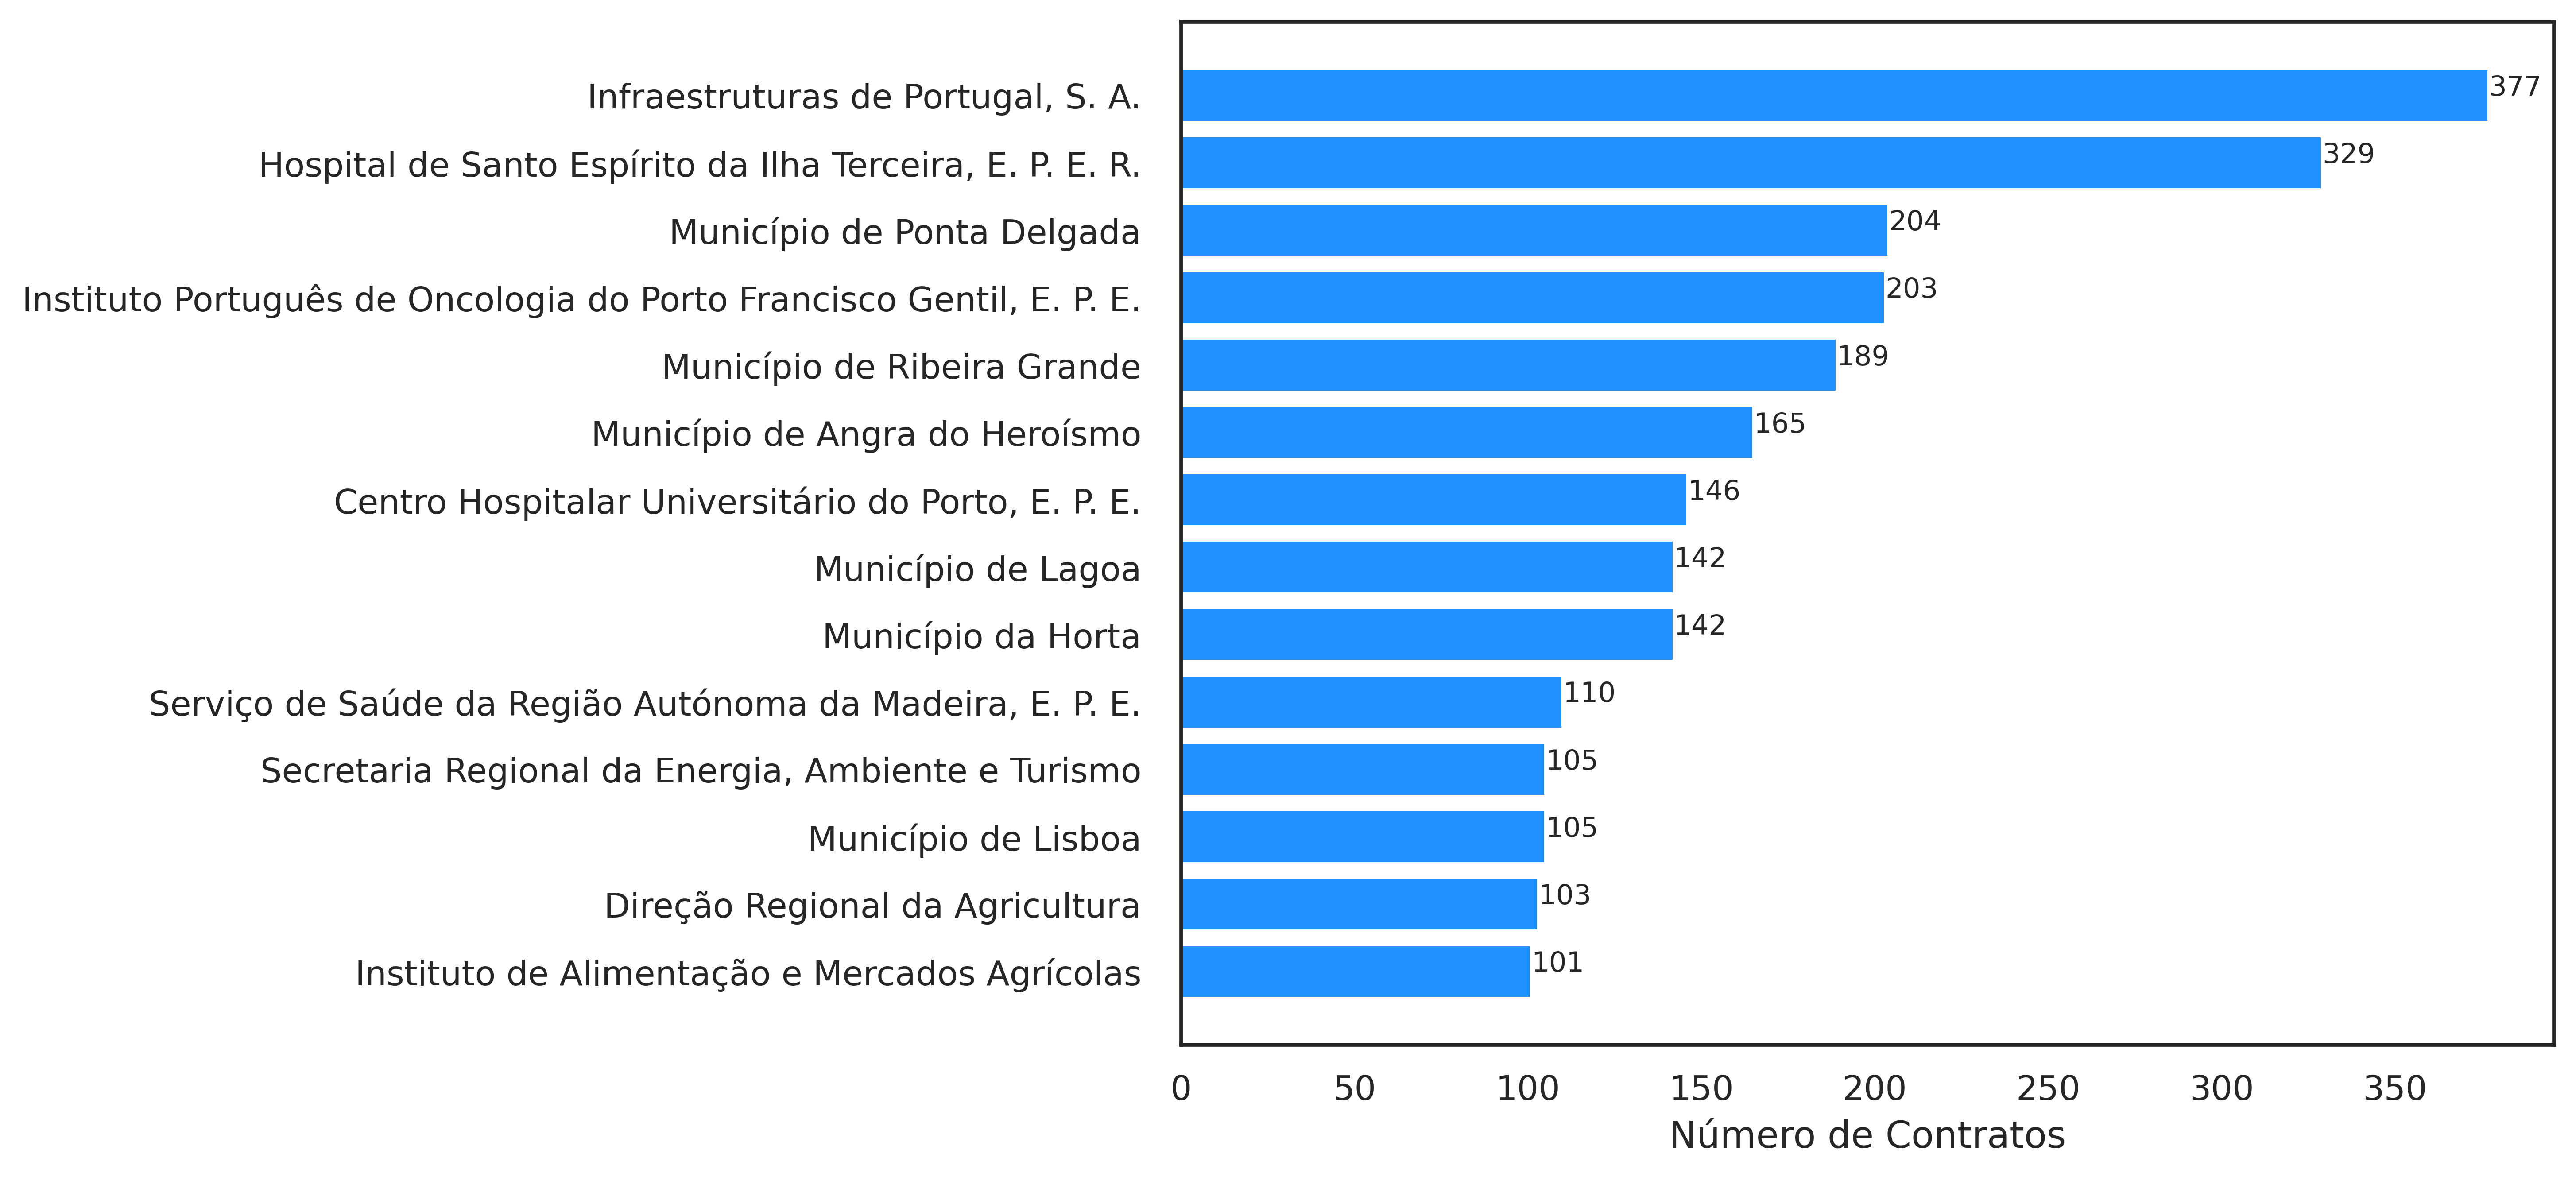
\includegraphics[width=\textwidth]{imagens/rf1/adjudicantes.png}
%	\caption{Entidades Adjudicantes com maior número de ajustes diretos celebrados em inconformidade com o CCP}
%	\label{}
%\end{figure}
%
%
%
%\begin{figure}[H]
%	\centering
%	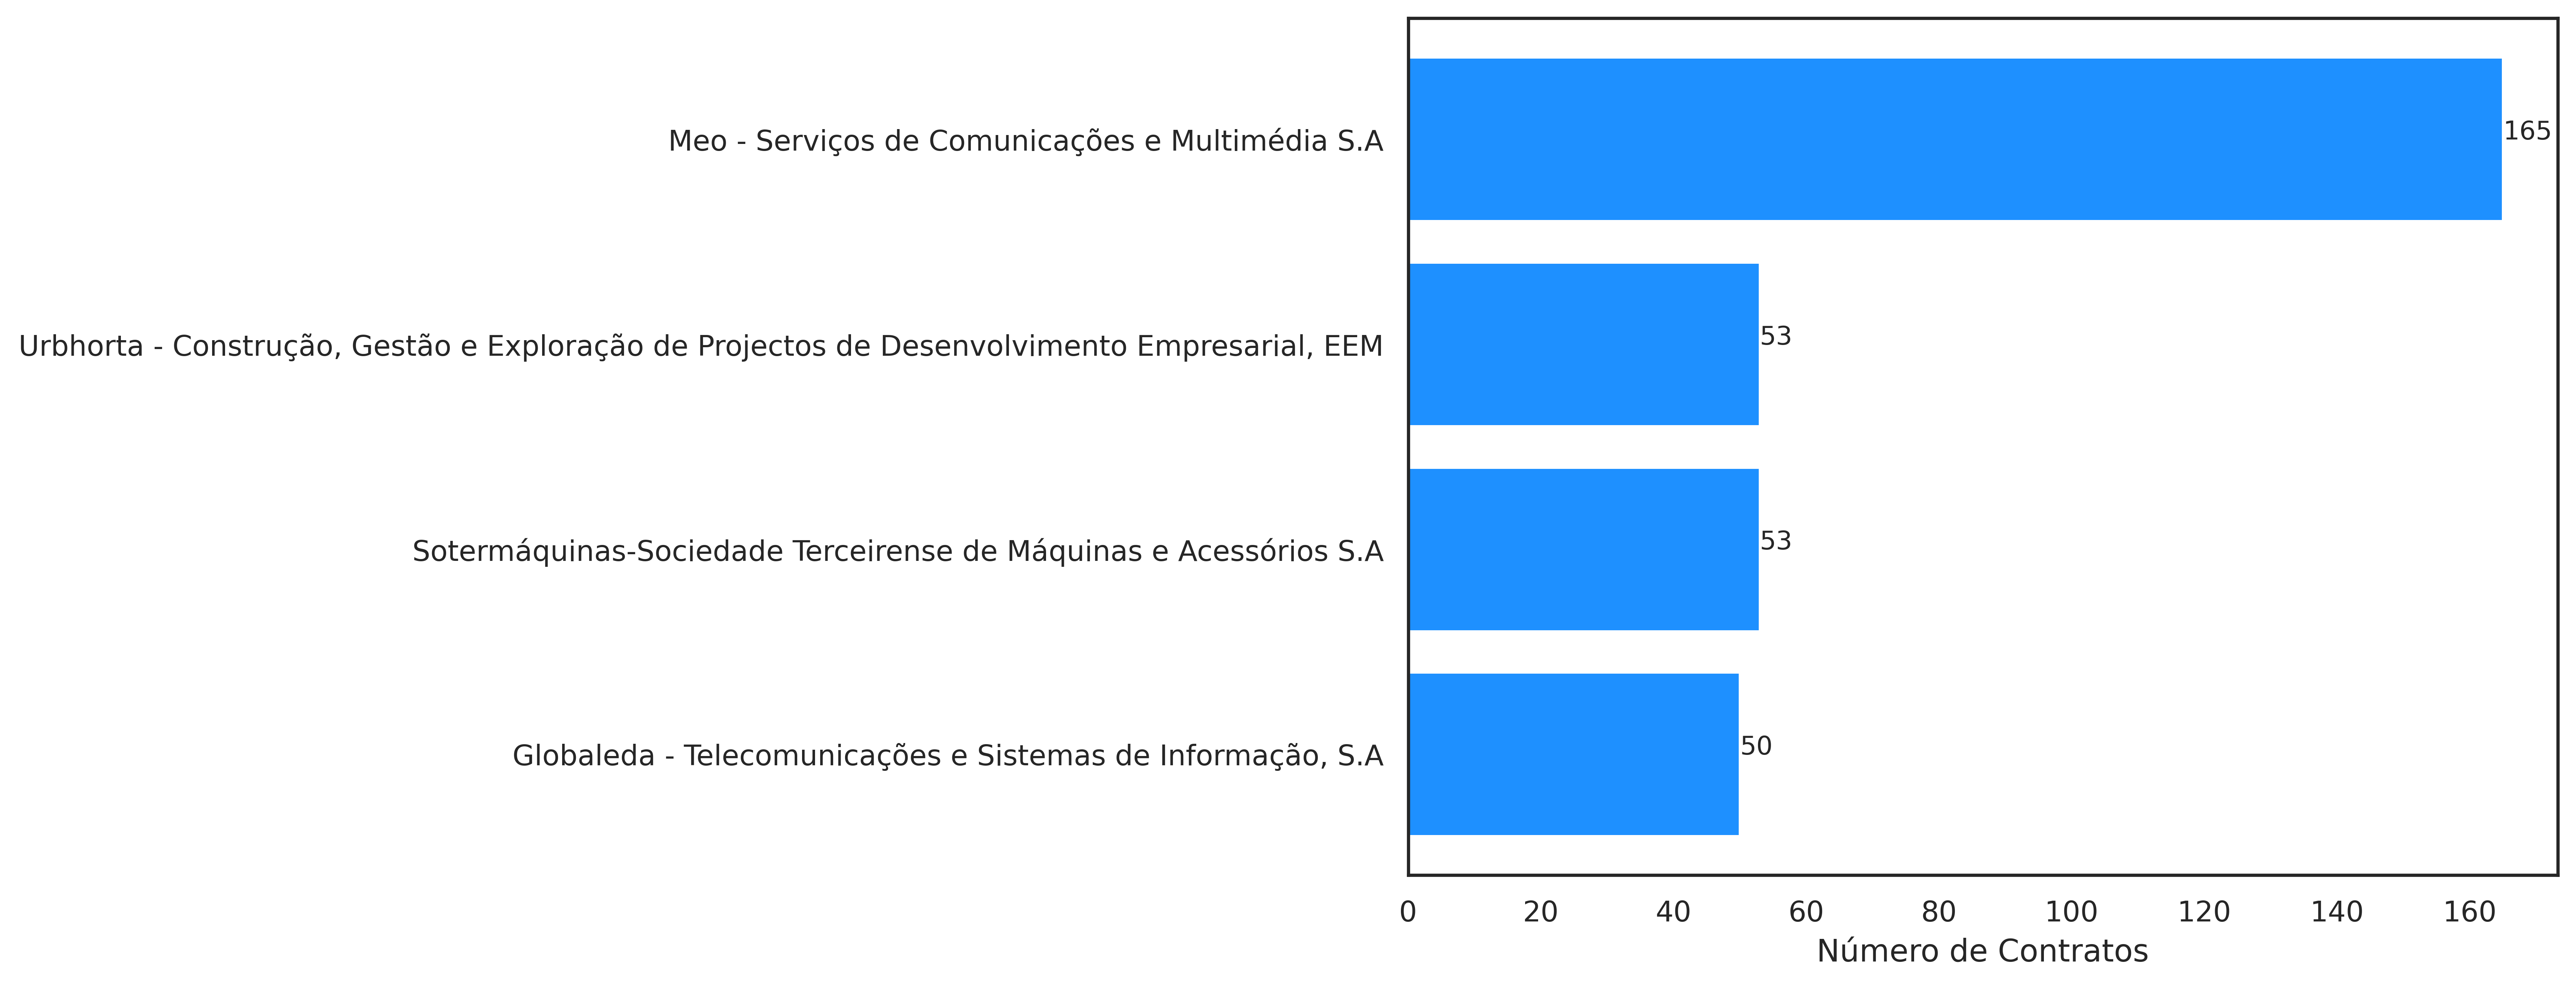
\includegraphics[width=\textwidth]{imagens/rf1/vencedora.png}
%	\caption{Entidades Adjudicantes com maior número de ajustes diretos celebrados em inconformidade com o CCP}
%	\label{}
%\end{figure}



\section{R003 : Análise do Prazo de Apresentação de Propostas}

Um factor importante ao longo da publicitação de um concurso público é o prazo disponível para que diferentes entidades interessadas possam efetuar propostas. Uma das flags definidas pela OCDS incide precisamente sobre esta questão.

\Lemma{}
{Short or inadequate notice to bidders to submit expressions of interest or bids. Bid period is less than expected (usually $\leq$2 days). The indicator should be calculated grouping by procurement method used, since the minimum bidding period might vary depending on the method.  It is important to check in local regulations if there is a minimun period.}


De acordo com o artigo 135.º do CCP - ver Tabela \ref{table:3} - o prazo mínimo para apresentação de propostas num concurso público para Bens e Serviços não pode ser inferior a 6 dias e, no caso de se tratar de um procedimento de formação de um contrato de empreitada de obras públicas, a 14 dias. Assim, para a construção desta flag, foi criada uma coluna adicional na tabela \textit{concursos\_publicos} chamada \textbf{tipo\_contrato}, tal como no indicador RF1. De seguida, foi construída uma \textit{query} para determinar todos os contratos referentes a concursos públicos que não respeitam estas condições apresentadas na Tabela mencionada. \\


\begin{lstlisting}[
	language=SQL,
	showspaces=false,
	showstringspaces=false,
	basicstyle=\ttfamily,
	numbers=left,
	numberstyle=\tiny,
	commentstyle=\color{gray}, frame = single,
	autogobble=true,
	breaklines=true,
	postbreak=\mbox{\textcolor{red}{$\hookrightarrow$}\space},
	]
	SELECT contratos_basegov."id" 
	FROM contratos_basegov
	JOIN concursos_publicos ON contratos_basegov."id" = concursos_publicos."id"
	WHERE (concursos_publicos."tipo_contrato" = 'Empreitadas' AND contratos_basegov."anuncio_proposalDeadline" < 14 AND contratos_basegov."anuncio_proposalDeadline" > 0) 
	OR
	(concursos_publicos."tipo_contrato" = 'Bens e Servicos' AND contratos_basegov."anuncio_proposalDeadline" < 6 AND
	contratos_basegov."anuncio_proposalDeadline" > 0);
	
\end{lstlisting}


Foi incluída uma condição adicional na \textit{query} para selecionar os contratos com prazo de apresentação de propostas superior a 0 dias. Esta condição foi imposta pois verificou-se que existiam alguns contratos com prazos negativos. Tendo em conta a dimensão dos valores - sempre superiores a 10, em módulo - inferiu-se que seriam erros de preenchimento aquando da inserção do contrato no Portal BASE e, como tal, não foram considerados. 

\begin{figure}[H]
	\centering
	\begin{minipage}{.48\linewidth}
		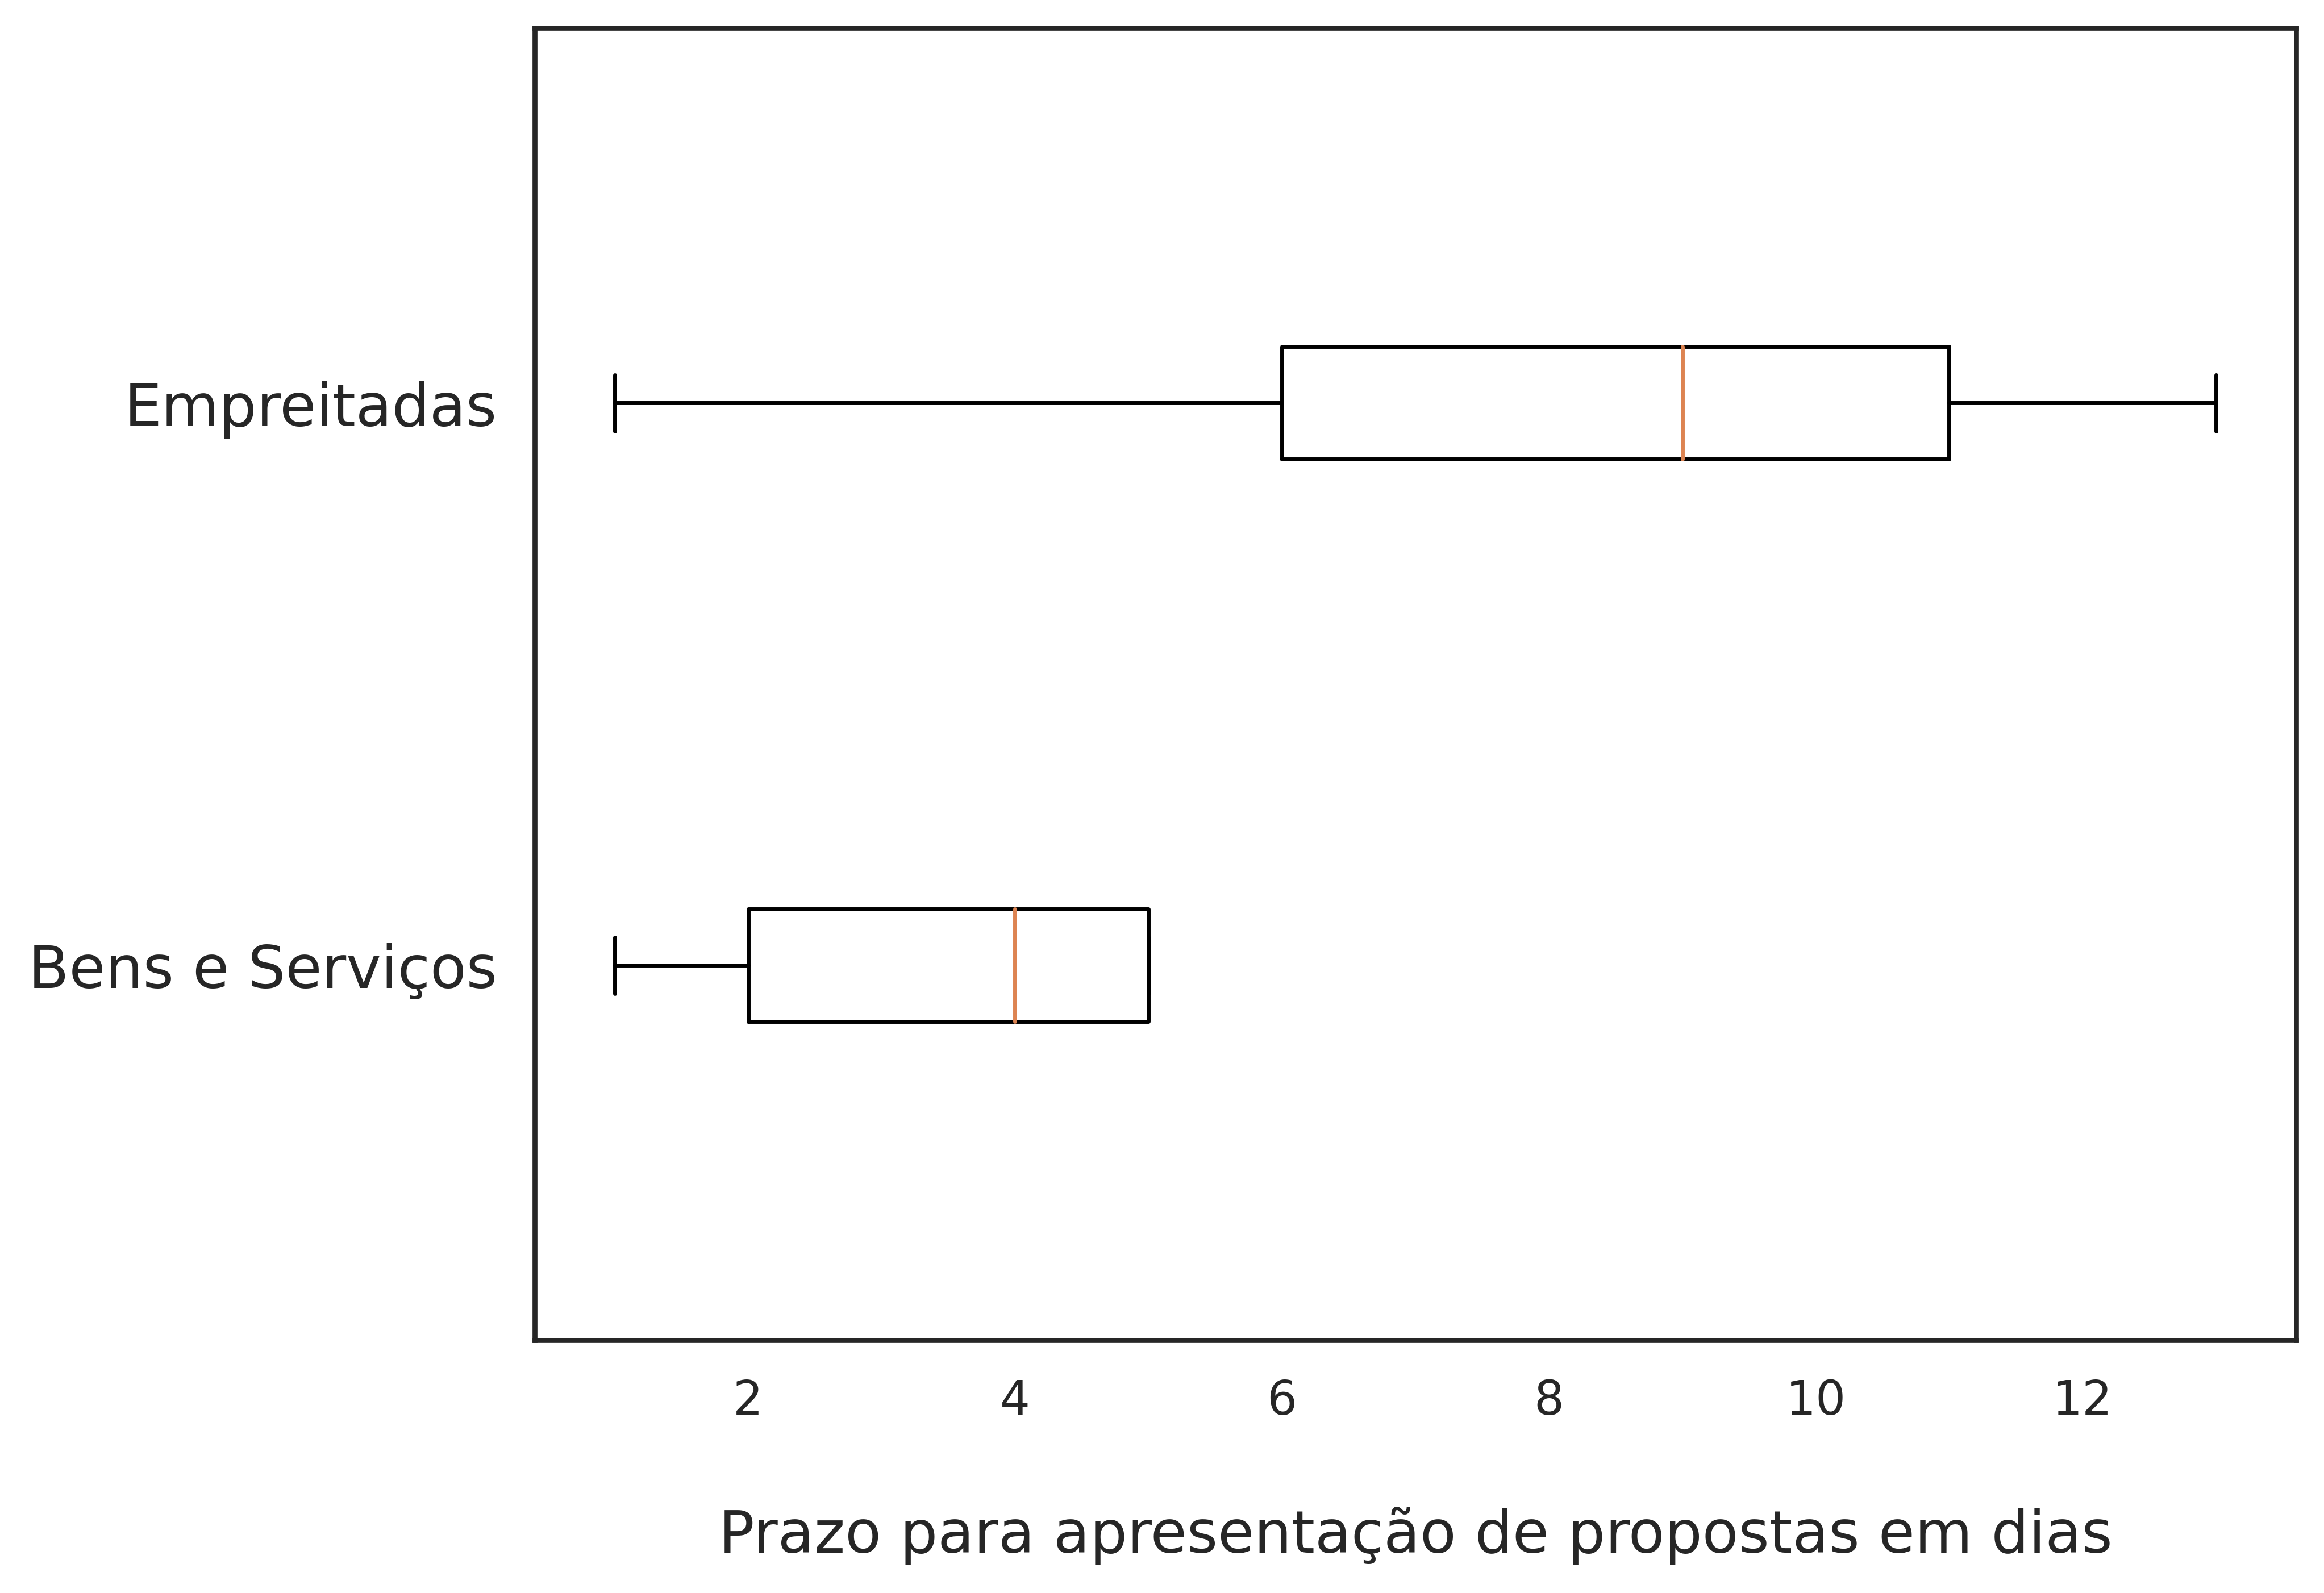
\includegraphics[width=\linewidth]{imagens/r003/boxplot_prazos.png}
		\caption{Distribuição do prazo de apresentação das propostas em dias para as duas tipologias de contratos.}
		
	\end{minipage}
	\hfill
	\begin{minipage}{.48\linewidth}
		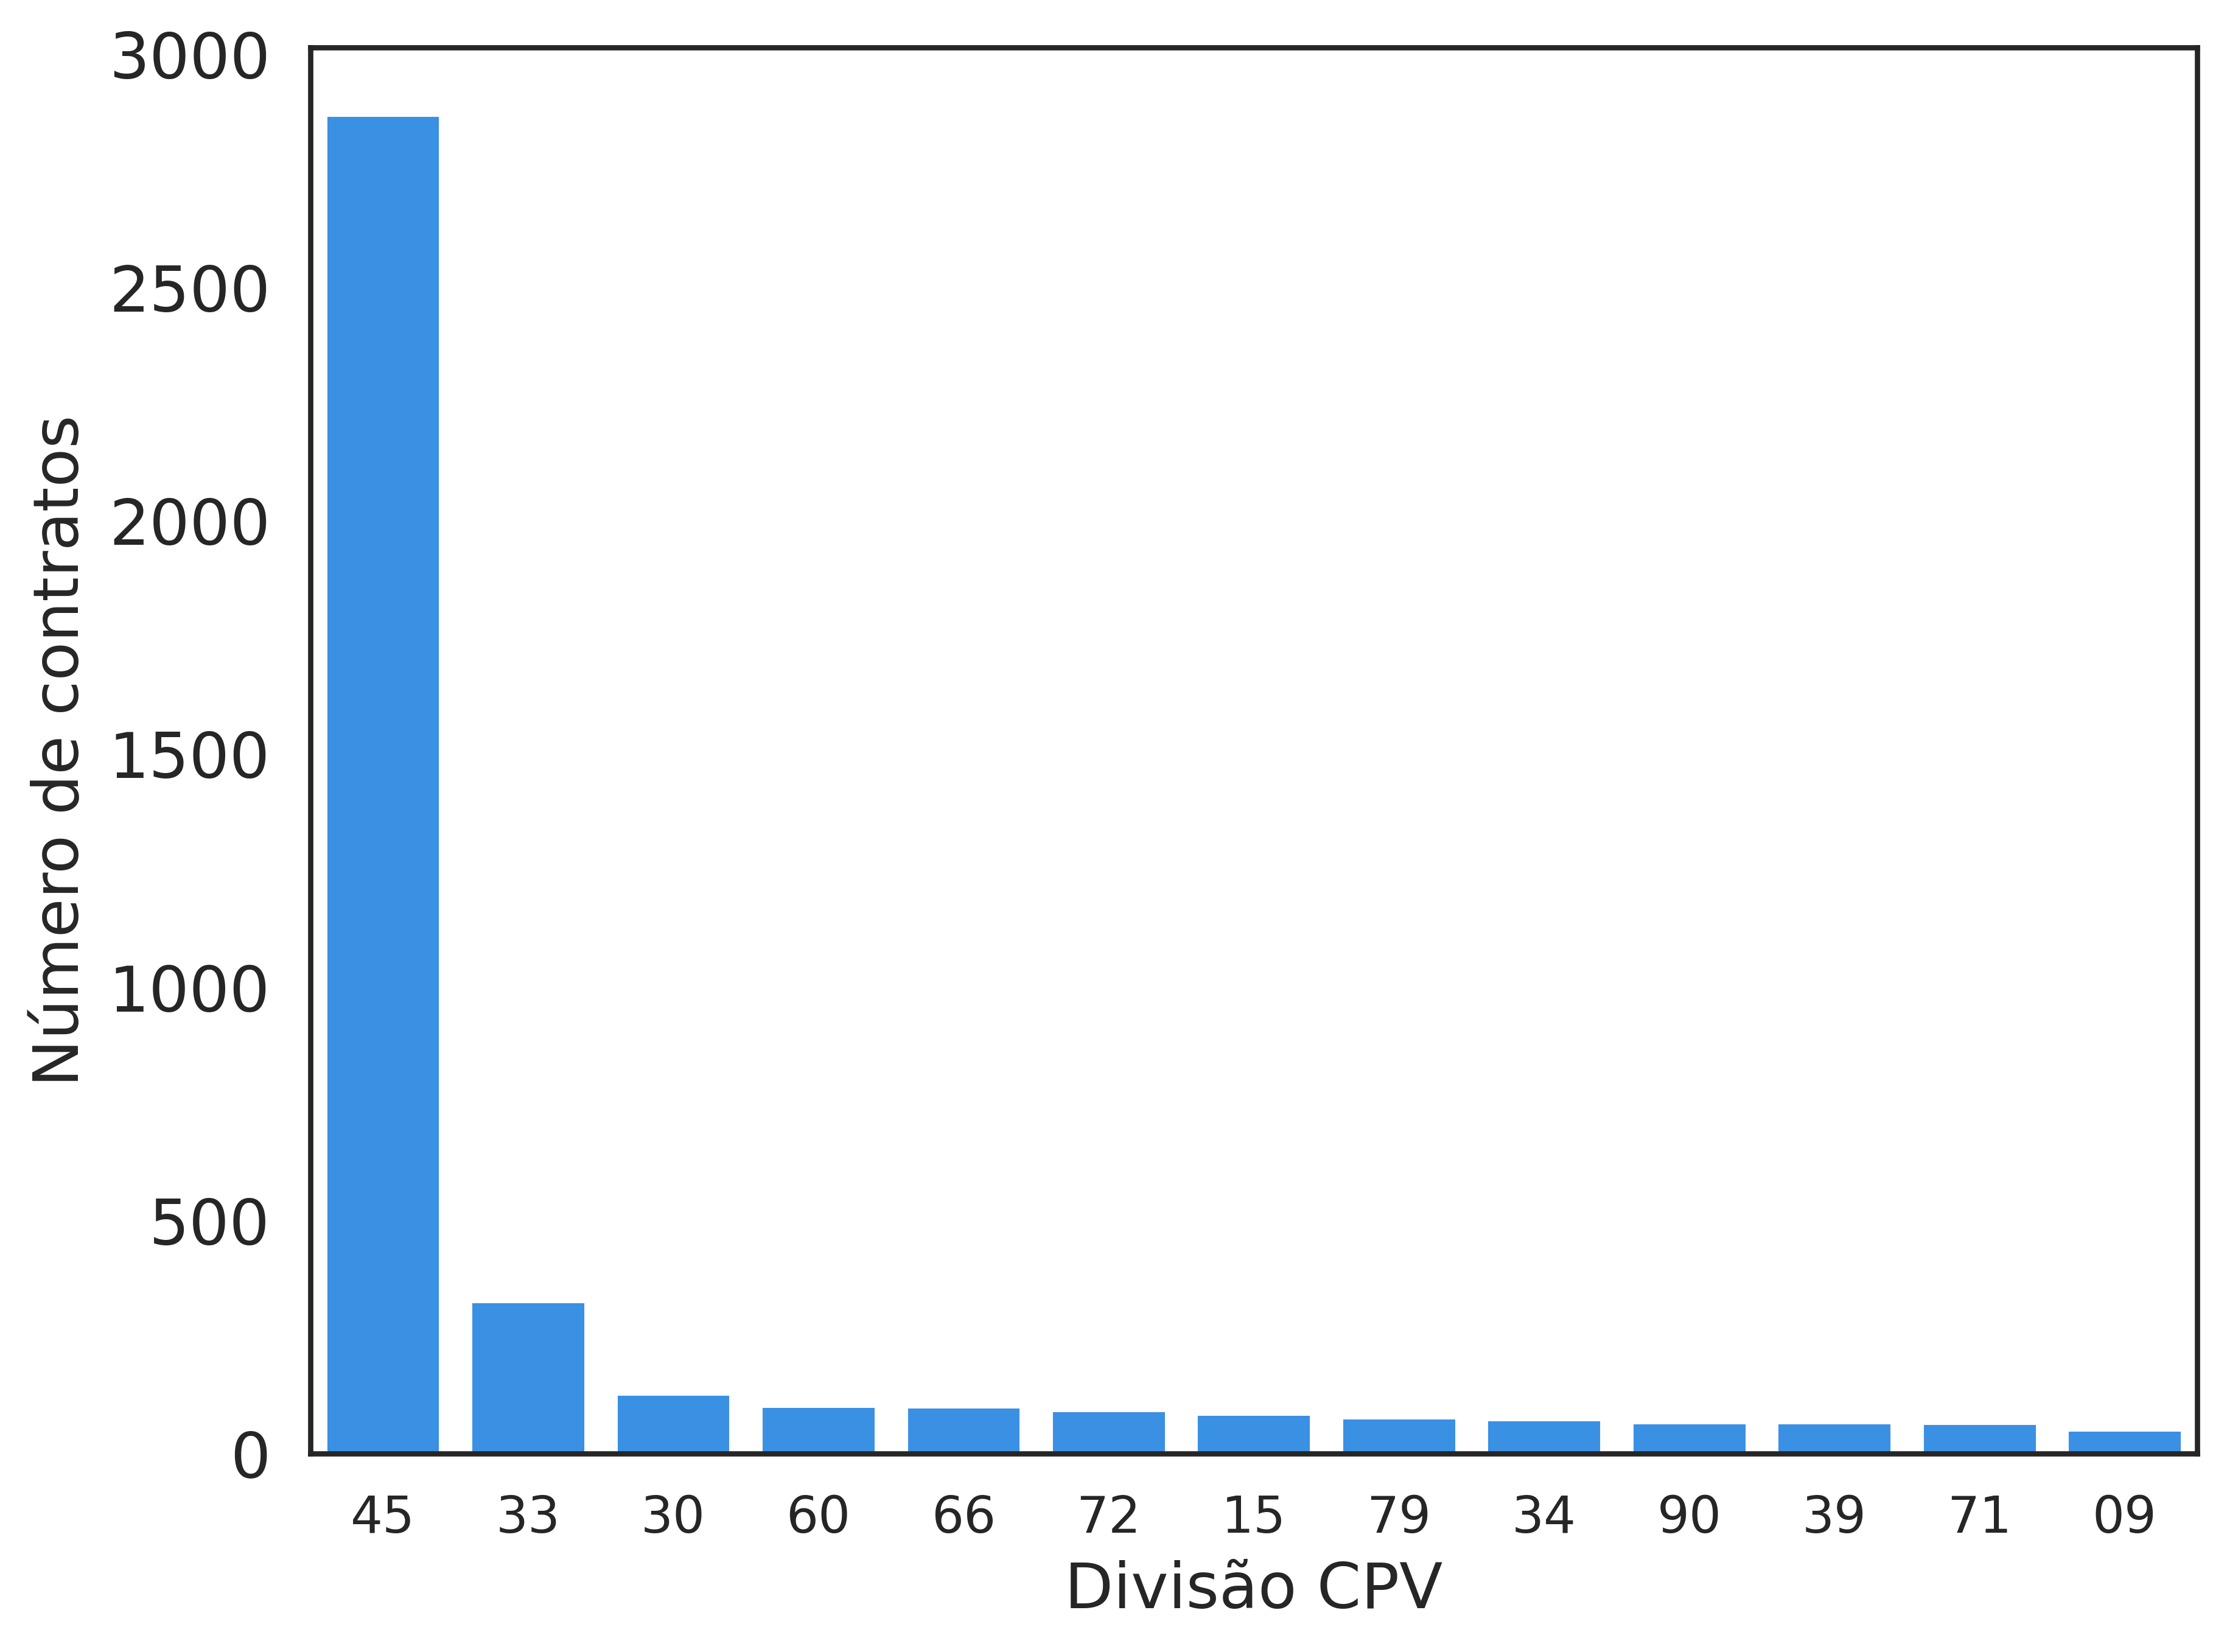
\includegraphics[width=\linewidth]{imagens/r003/main_cpvs.png}
		\caption{Principais divisões de CPV com maior número de contratos em trangressão.}
		
	\end{minipage}
\end{figure}

É na divisão da Construção Civil onde se verifica a existência de um maior incumprimento do prazo mínimo de dias para apresentação de propostas, atingindo uma percentagem de 70\% dos contratos inconformes. Perante a totalidade de concursos públicos celebrados referentes a construção civil, esta percentagem é de 13\%.


\subsection{R017 : Comparação do Preço Contratual com Preço Médio por CPV}


\Lemma{}
{
	The difference between an item value and its expected value is above a threshold. 
}

Para construção deste indicador foi calculado o preço médio por CPV. O conjunto de contratos foi agrupado pelos primeiros três dígitos - grupo - do CPV de forma a obter um maior nível de granularidade. Para cada um dos 302 grupos foi calculado o preço contratual médio, desvio padrão, mínimo, máximo e primeiro, segundo e terceiro quartis. O resultado obtido assemelha-se à seguinte tabela : 


\begin{table}[h!]
	
	\setlength\tabcolsep{1pt}
	\begin{tabular*}{\linewidth}{@{\extracolsep{\fill}} |c|c|c|c|c|c|c|c|c|c|}
		\hline
		\textbf{cpv3} & \textbf{preco\_total} & \textbf{count} & \textbf{mean} & \textbf{std} & \textbf{min} & \textbf{q1} & \textbf{q2} & \textbf{q3} & \textbf{max} \\ \hline
		641           & 6700942.8           & 57             & 117560.4    & 179755.1   & 1575         & 10639.2     & 60000       & 165892.2    & 885500       \\ \hline
	\end{tabular*}
	\caption{Primeira linha da tabela auxiliar construída}
	
\end{table}


Contudo, a partir da construção desta tabela, constatou-se que, certamente devido a erros de preenchimento na plataforma BaseGOV, existem inúmeros valores de preço contratuais com valores negativos ou com valor nulo. Desta forma, o valor médio calculado não corresponde ao verdadeiro valor médio e, como tal, a comparação que se pretendia efetuar na próxima etapa deste indicador entre o preço contratual e o preço médio contratual por grupo é inapropriada. 

\subsection{R018 : Análise de Contratos com uma entidade concorrente}

Um dos parâmetros importantes a ter em conta ao analisar um contrato público prende-se com o número de entidades concorrentes. A partir deste ponto, podem ser analisadas três situações distintas ao longo do processo contratual: 
quando apenas se candidatou uma entidade,quando se candidatou um \textit{elevado} número de entidades,quando se candidatou um \textit{baixo} número de entidades. Comecemos pela primeira, definida da seguinte forma pela OCDS:

\Lemma{}
{Single bid received : Tender featured a single bidder only }


Dado que uma das colunas da tabela diz respeito às entidades que se candidataram a um determinado concurso, pode ser feita uma análise do número de entidades concorrentes. Esta coluna é preenchida de uma forma análoga ao representado na Tabela \ref{tab:entsconc}. 


\begin{table}[H]
	\centering
	\begin{tabular}{|c|c|}
		\hline
		\textbf{ID}   & \textbf{EntidadesConcorrentes}                                                                                                      \\ \hline
		$\text{ID}_1$ & $\text{Entidade}\_i$ ( $\text{NIF}\_i$) $|||$ $\text{Entidade}\_j$ ( $\text{NIF}\_j$)                                               \\ \hline
		$\text{ID}_2$ & $\text{Entidade}\_k$ ( $\text{NIF}\_k$)                                                                                             \\ \hline
		$\dots$       & $\dots$                                                                                                                             \\ \hline
		$\text{ID}_n$ & $\text{Entidade}\_l$ ( $\text{NIF}\_l$) $|||$ $\text{Entidade}\_m$ ( $\text{NIF}\_m$) $|||$ $\text{Entidade}\_n$ ( $\text{NIF}\_n$) \\ \hline
	\end{tabular}
	\caption{Formato da coluna entidades\_concorrentes}
	\label{tab:entsconc}
\end{table}

Para cada entidade que concorre, é inserido o respetivo nome e número de identificação fiscal (NIF) e, na eventualidade do número de entidades concorrentes ser superior a 1, a separação entre as mesmas é feita recorrendo a um separador $|||$. Desta forma, foi necessário desenvolver uma \textit{query} que conta o número de elementos separados e insira o resultado desta contagem numa nova coluna criada, chamada \textit{nr\_entidadesconcorrentes}.


\begin{lstlisting}[
	language=SQL,
	showspaces=false,
	basicstyle=\ttfamily,
	numbers=left,
	numberstyle=\tiny,
	commentstyle=\color{gray}, frame = single,
	breaklines=true,
	autogobble =true,
	postbreak=\mbox{\textcolor{red}{$\hookrightarrow$}\space},
	]
	UPDATE concursospublicos
	SET nr_entidadesconcorrentes = ARRAY_LENGTH(STRING_TO_ARRAY( entidades_concorrentes, '|||'), 1) + 1;	
\end{lstlisting}

Através desta nova coluna, é possível selecionar todos os contratos que apenas contemplem uma entidade concorrente. 

\begin{lstlisting}[
	language=SQL,
	showspaces=false,
	basicstyle=\ttfamily,
	numbers=left,
	numberstyle=\tiny,
	commentstyle=\color{gray}, frame = single,
	breaklines=true,
	autogobble =true,
	postbreak=\mbox{\textcolor{red}{$\hookrightarrow$}\space},
	]
	SELECT contratos_basegov."id"
	FROM contratos_basegov
	JOIN concursos_publicos ON contratos_basegov."id" = concursos_publicos."id"
	WHERE concursos_publicos."nr_entidadesconcorrentes" = 1;
\end{lstlisting}


\begin{figure}[H]
	\centering
	\begin{minipage}{.48\linewidth}
		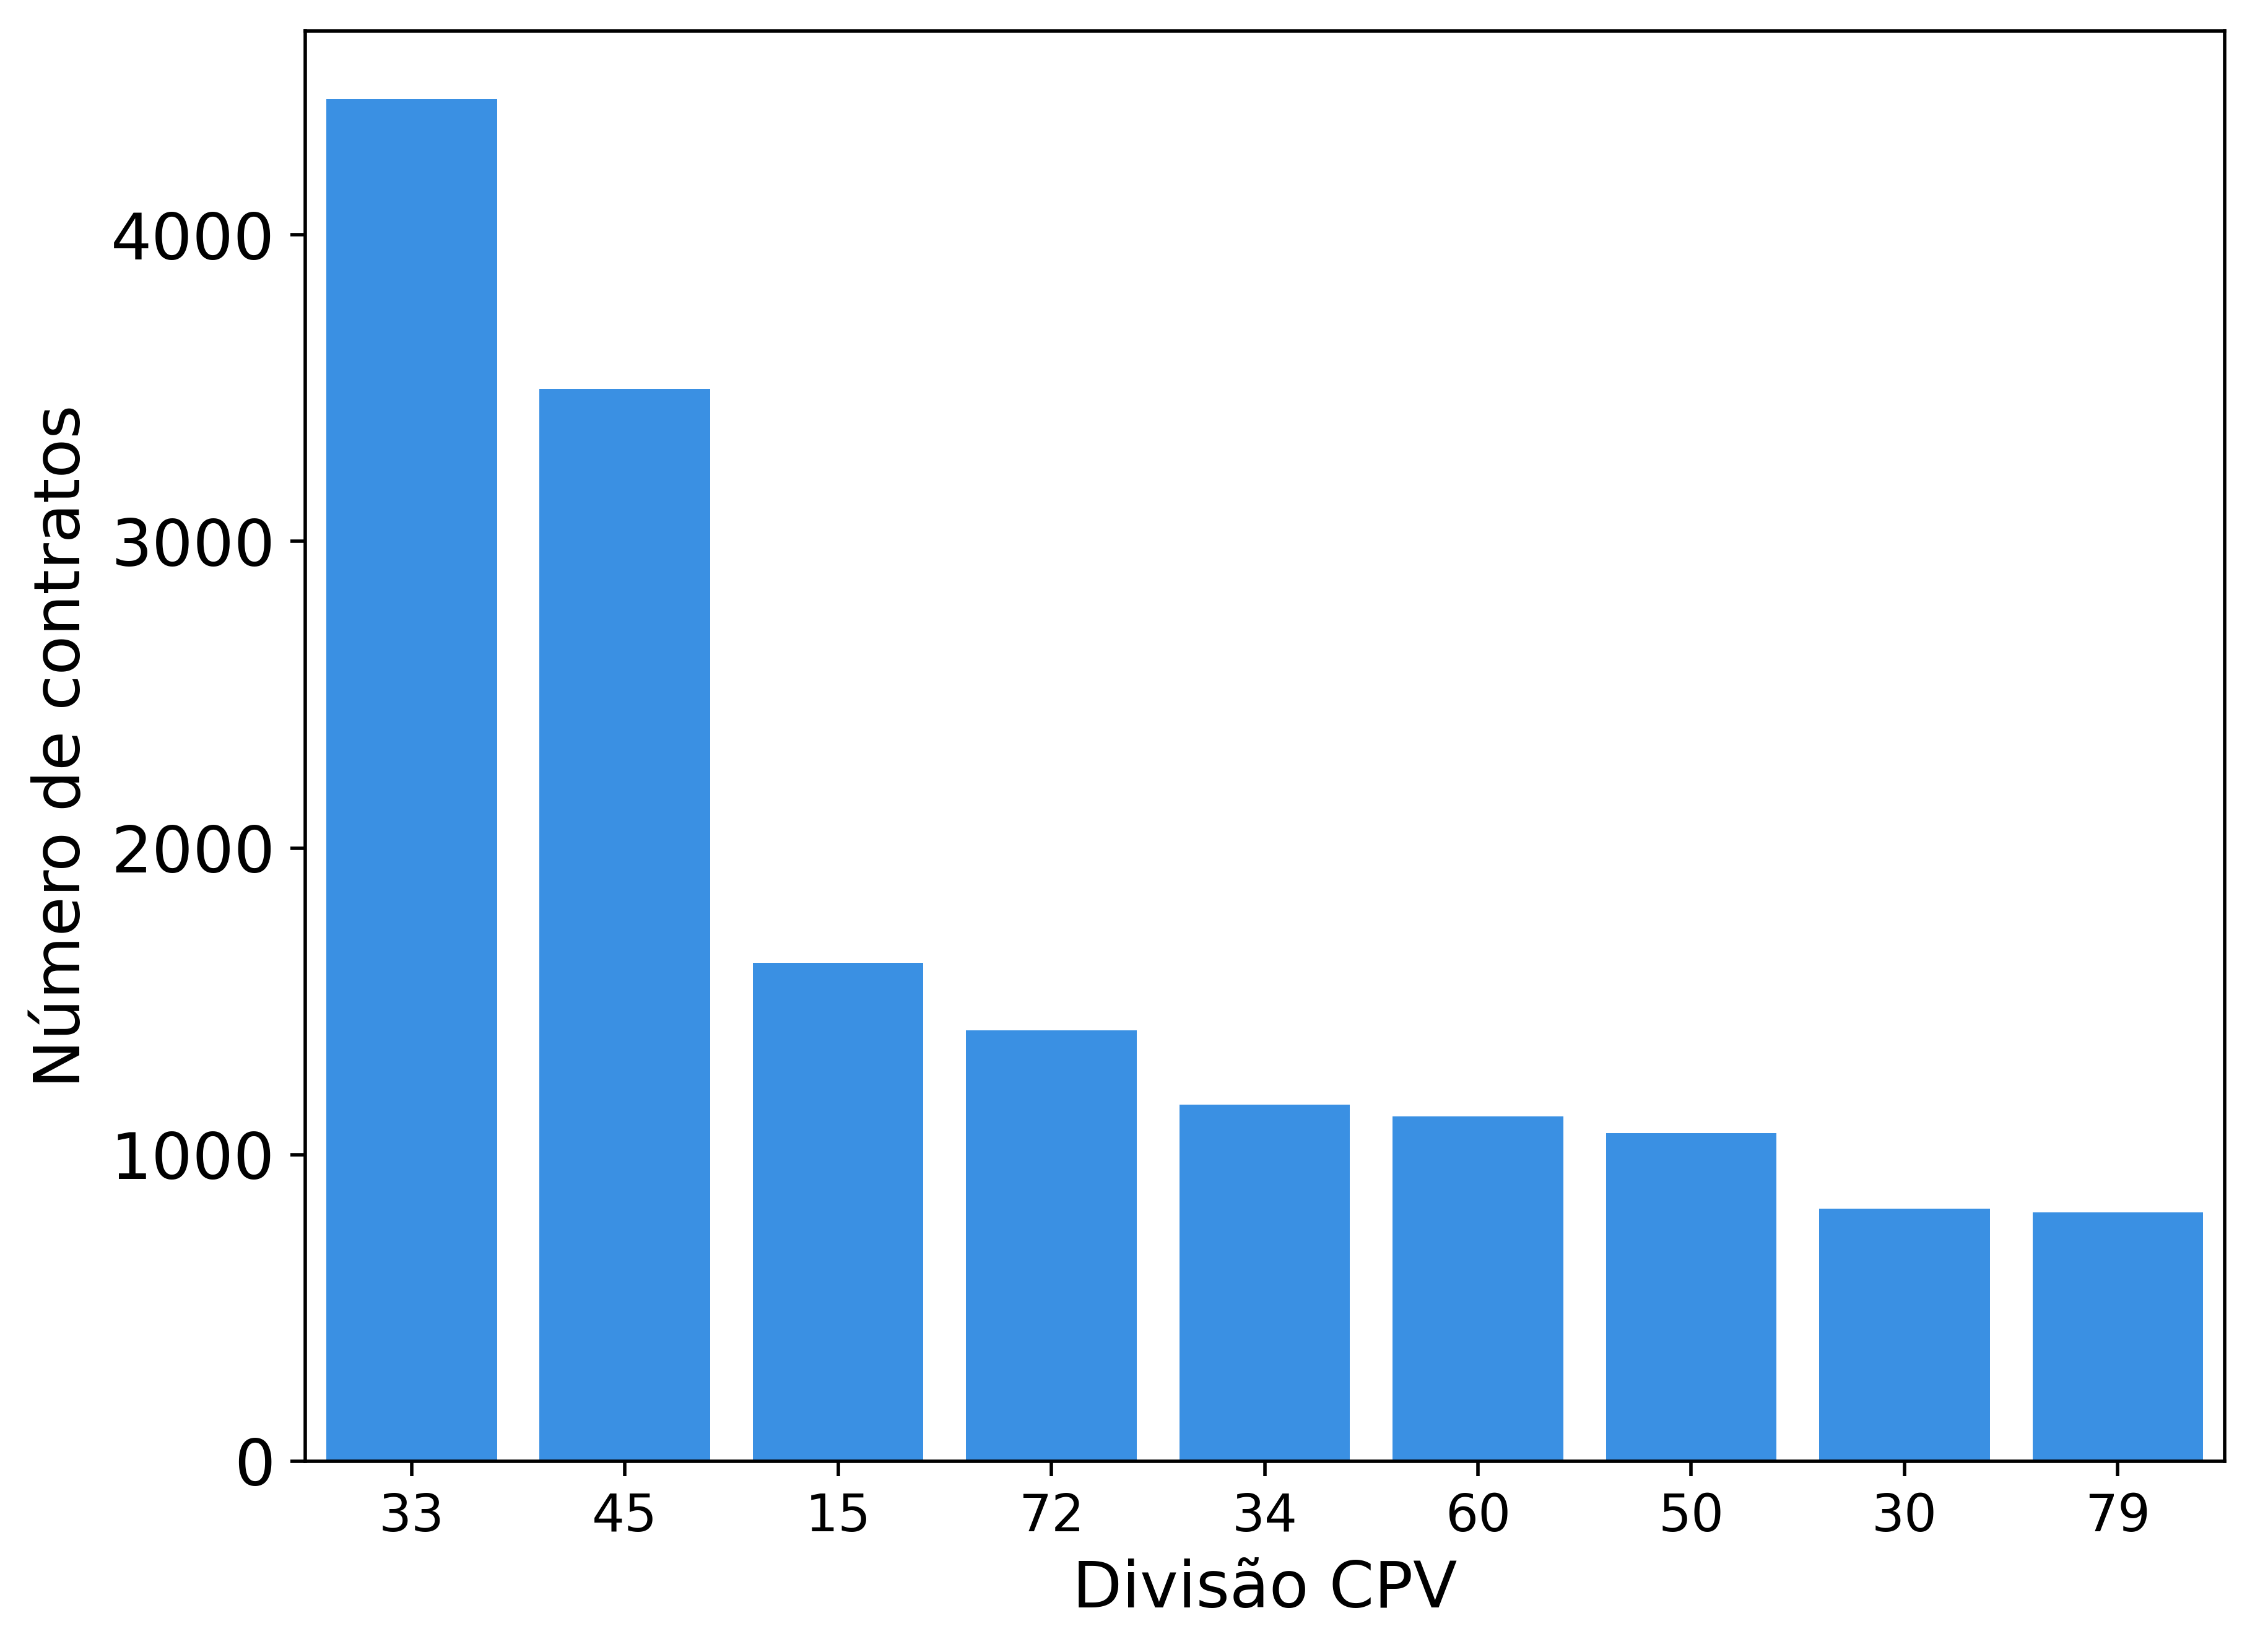
\includegraphics[width=\linewidth]{imagens/r018/main_cpvs.png}
		\caption{Divisões de CPV com maior número de contratos em inconformidade.}
	\end{minipage}
	\hfill
	\begin{minipage}{.49\linewidth}
		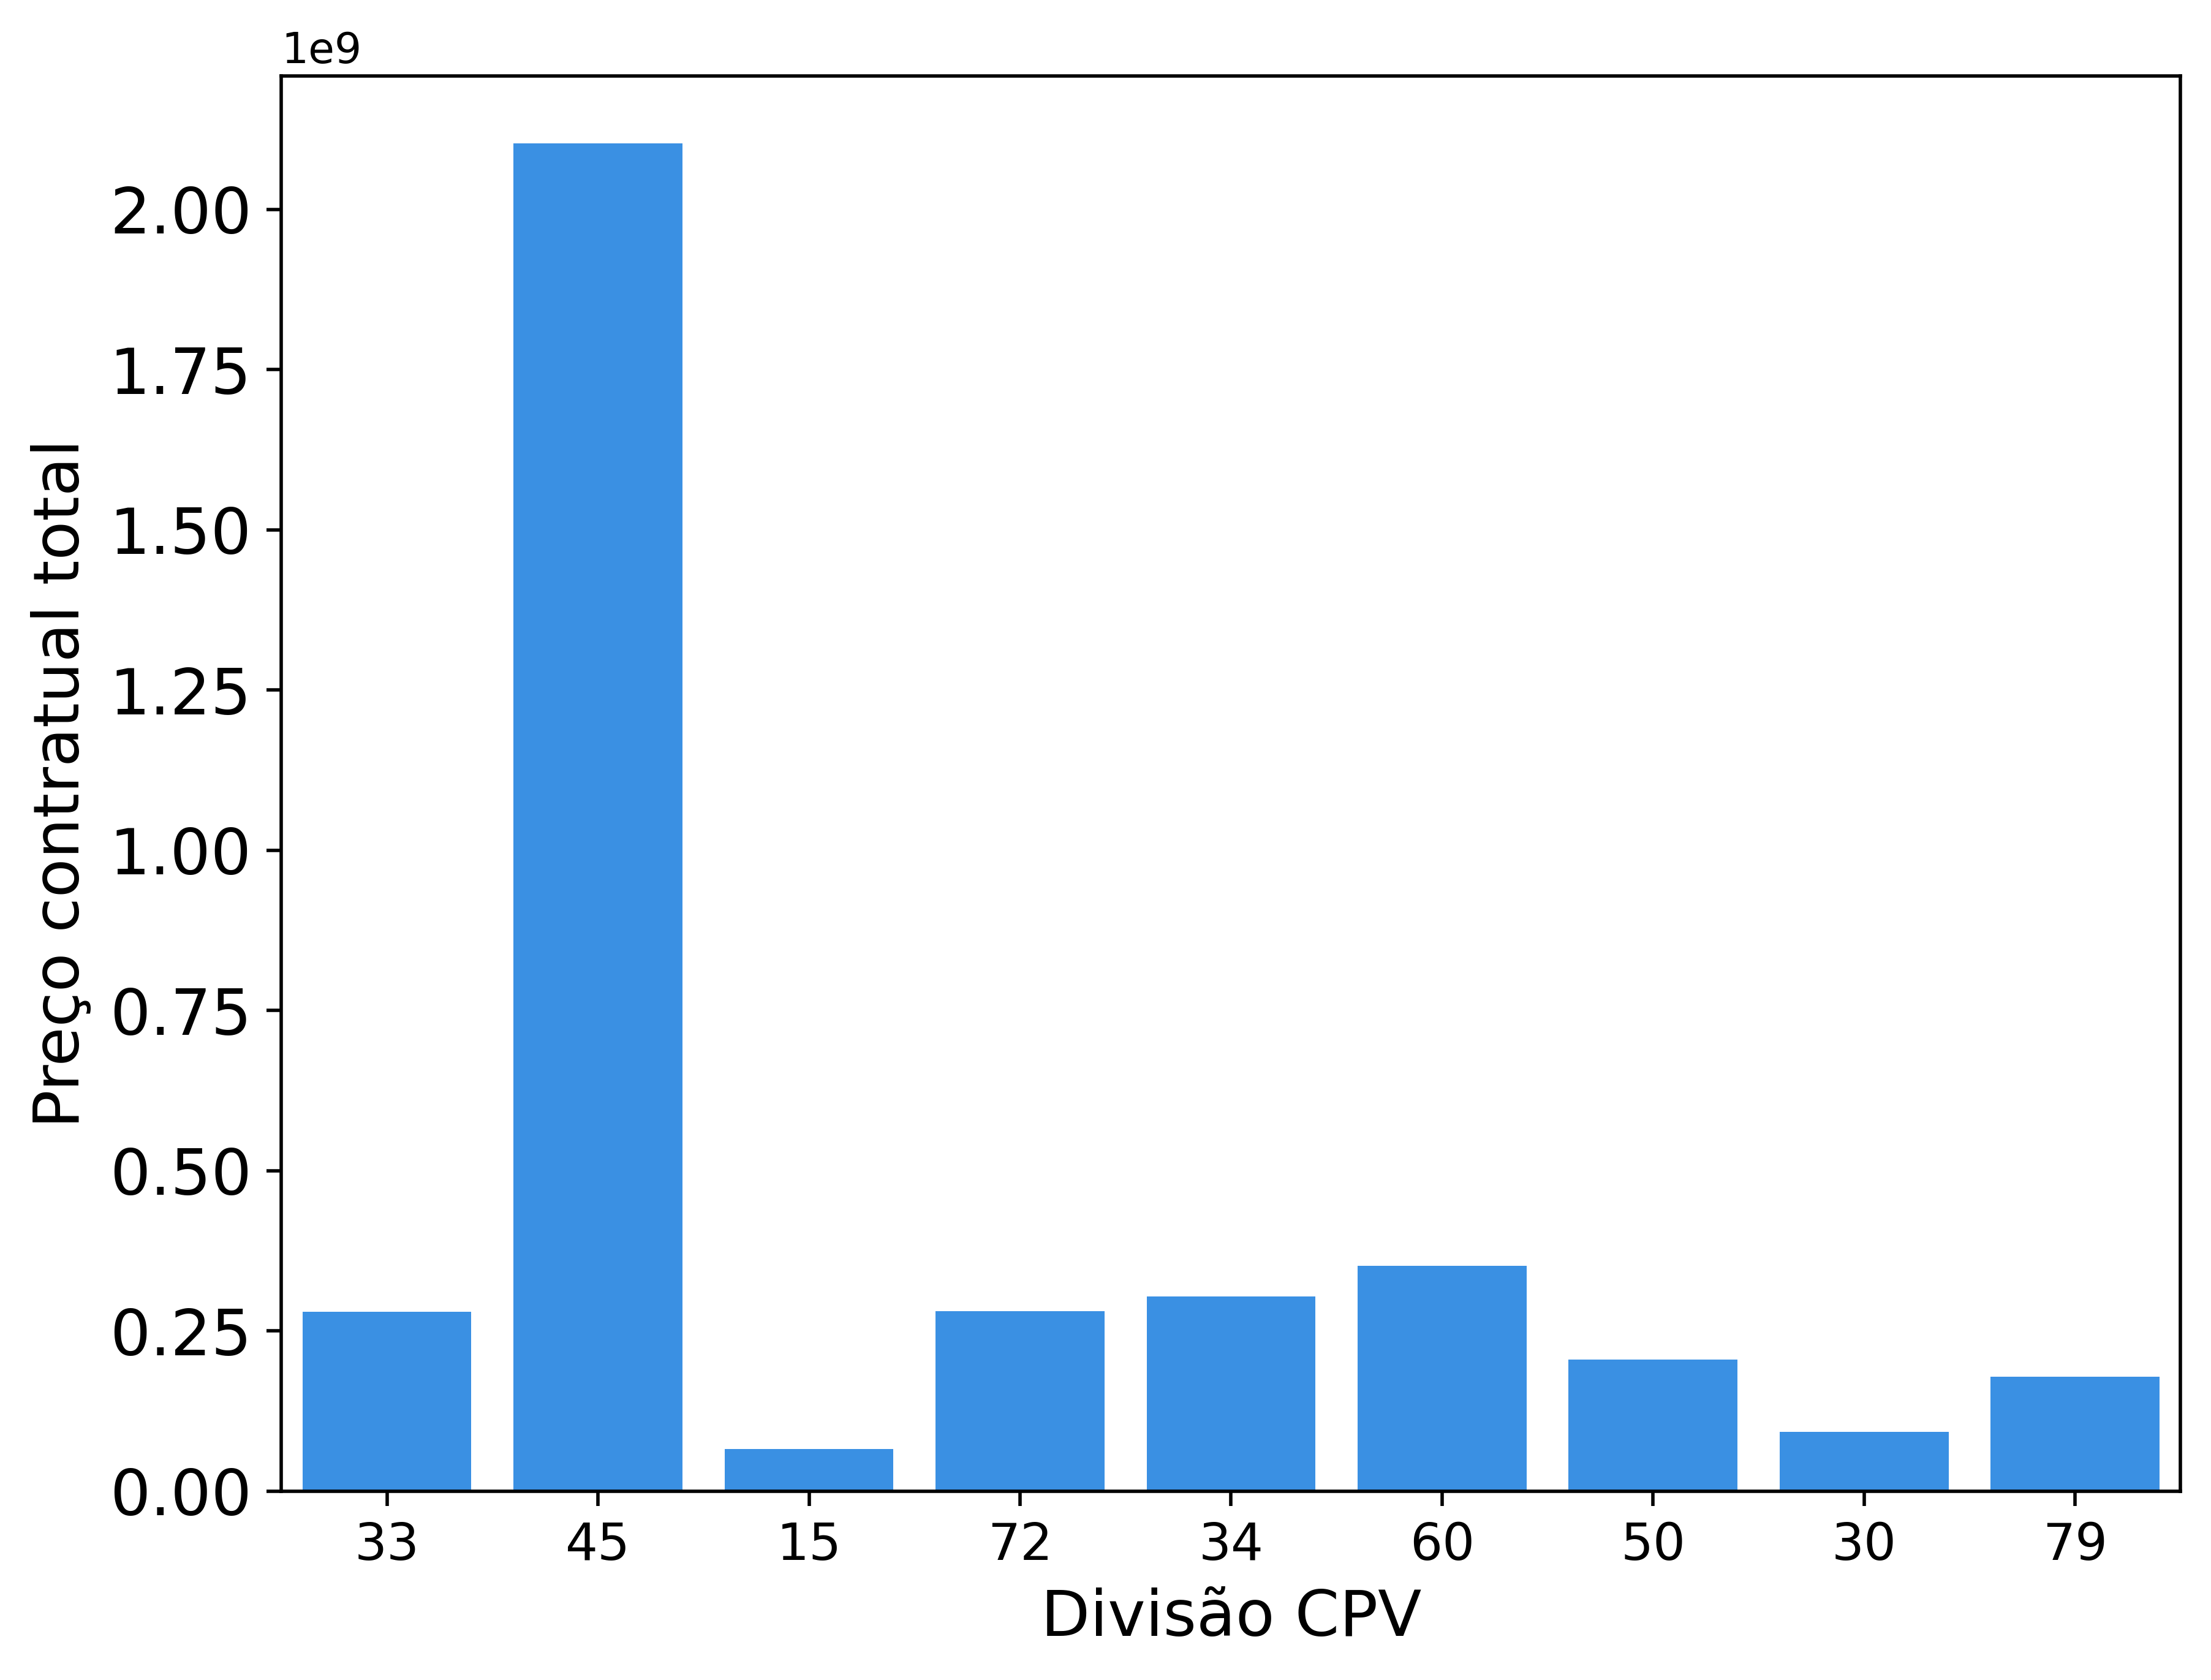
\includegraphics[width=\linewidth]{imagens/r018/prices.png}
		\caption{Valor adjudicado total para todos dos contratos em inconformidade para divisão de CPV.}
	\end{minipage}
\end{figure}




\begin{table}[H]
	\centering
	\renewcommand{\arraystretch}{1.15}
	\setlength{\tabcolsep}{15pt}
	\resizebox{\textwidth}{!} & \textbf{\begin{tabular}[c]{@{}c@{}}Número de \\ contratos total\end{tabular}} & \textbf{\%} & \textbf{\begin{tabular}[c]{@{}c@{}}Preço contratual\\ total\end{tabular}} \\ \hline
		33                   & 4444                                                                                & 27          & 29351                                                                         & 15.1        & 279.688.414,00€                                                           \\
		45                   & 3498                                                                                & 22          & 21525                                                                         & 16.3        & 2.103.391.451,00€                                                         \\
		15                   & 1625                                                                                & 10          & 5963                                                                          & 27.2        & 280.726.463,00€                                                           \\
		72                   & 1406                                                                                & 9           & 3739                                                                          & 37.6        & 65.760.473,00€                                                            \\
		34                   & 1162                                                                                & 7           & 4597                                                                          & 25.3        & 303.614.946,00€                                                           \\
		60                   & 1124                                                                                & 7           & 3512                                                                          & 32          & 351.923.997,00€                                                           \\
		50                   & 1069                                                                                & 6           & 3908                                                                          & 27.4        & 205.240.508,00€                                                           \\ \midrule
		\textbf{Total}       & 14328                                                                               & -           & 72595                                                                         & -           & -                                                                         \\ \hline
	\end{tabular}%
	}
	\caption{Descrição do número de contratos, total e inconformes, para as principais divisões de CPV.}
	\label{tab:rf18stats}
\end{table}







\subsection{R019 : Análise do Número de Entidades Concorrentes}

\Lemma{}
	{
	Low number of bidders for item and procuring entity. Number of bidders significantly less than average, based on prior similar contracts (for similar item or procuring entity) 
	}


Para a construção deste indicador, foi necessário construir uma tabela adicional. Para cada uma das 46 divisões de CPV, foi feita uma contagem de todos os contratos, calculado o número total de entidades concorrentes de entre todos os contratos e foram calculados os seguintes indicadores estatísticos : média, desvio-padrão, primeiro-quartil, segundo-quartil, terceiro-quartil, mínimo e máximo. Este procedimento foi feito através de um script \textit{python}, obtendo-se uma tabela do género : 

\begin{table}[H]
	\centering
	\begin{tabular}{|c|c|c|c|c|c|c|c|c|c|}
		\hline
		\textbf{cpv} & \textbf{nec\_t} & \textbf{count} & \textbf{mean} & \textbf{std} & \textbf{min} & \textbf{q1} & \textbf{q2} & \textbf{q3} & \textbf{max} \\ \hline
		98           & 1739            & 586            & 2.968         & 2.251        & 1            & 1           & 2           & 4           & 15           \\ \hline
	\end{tabular}
	\caption{}
\end{table}

sendo que \textbf{cpv} corresponde a cada umas das divisões de CPV, \textit{nec\_t} corresponde ao número total de entidades concorrentes em todos os concursos, \textit{count} é número total de contratos, \textbf{mean}, \textbf{std}, \textbf{min}, \textbf{q1}, \textbf{q2}, \textbf{q3} e \textbf{max} são, respetivamente, o valor médio, o desvio padrão, mínimo, primeiro quartil, segundo quartil, terceiro quartil e máximo para todos os contratos cujos primeiros dois digitos do CPV sejam iguais aos da primeira coluna. 

Com o resultado obtido, foi feita, numa primeira instância, uma representação gráfica dos valores da média, mediana e desvio-padrão, por CPV, a fim de ter uma ideia da dispersão - distância entre a média e o desvio padrão - e simetria da distribuição - distância entre média e mediana - dos preços contratuais.

\begin{figure}[!htbp]
	\centering
	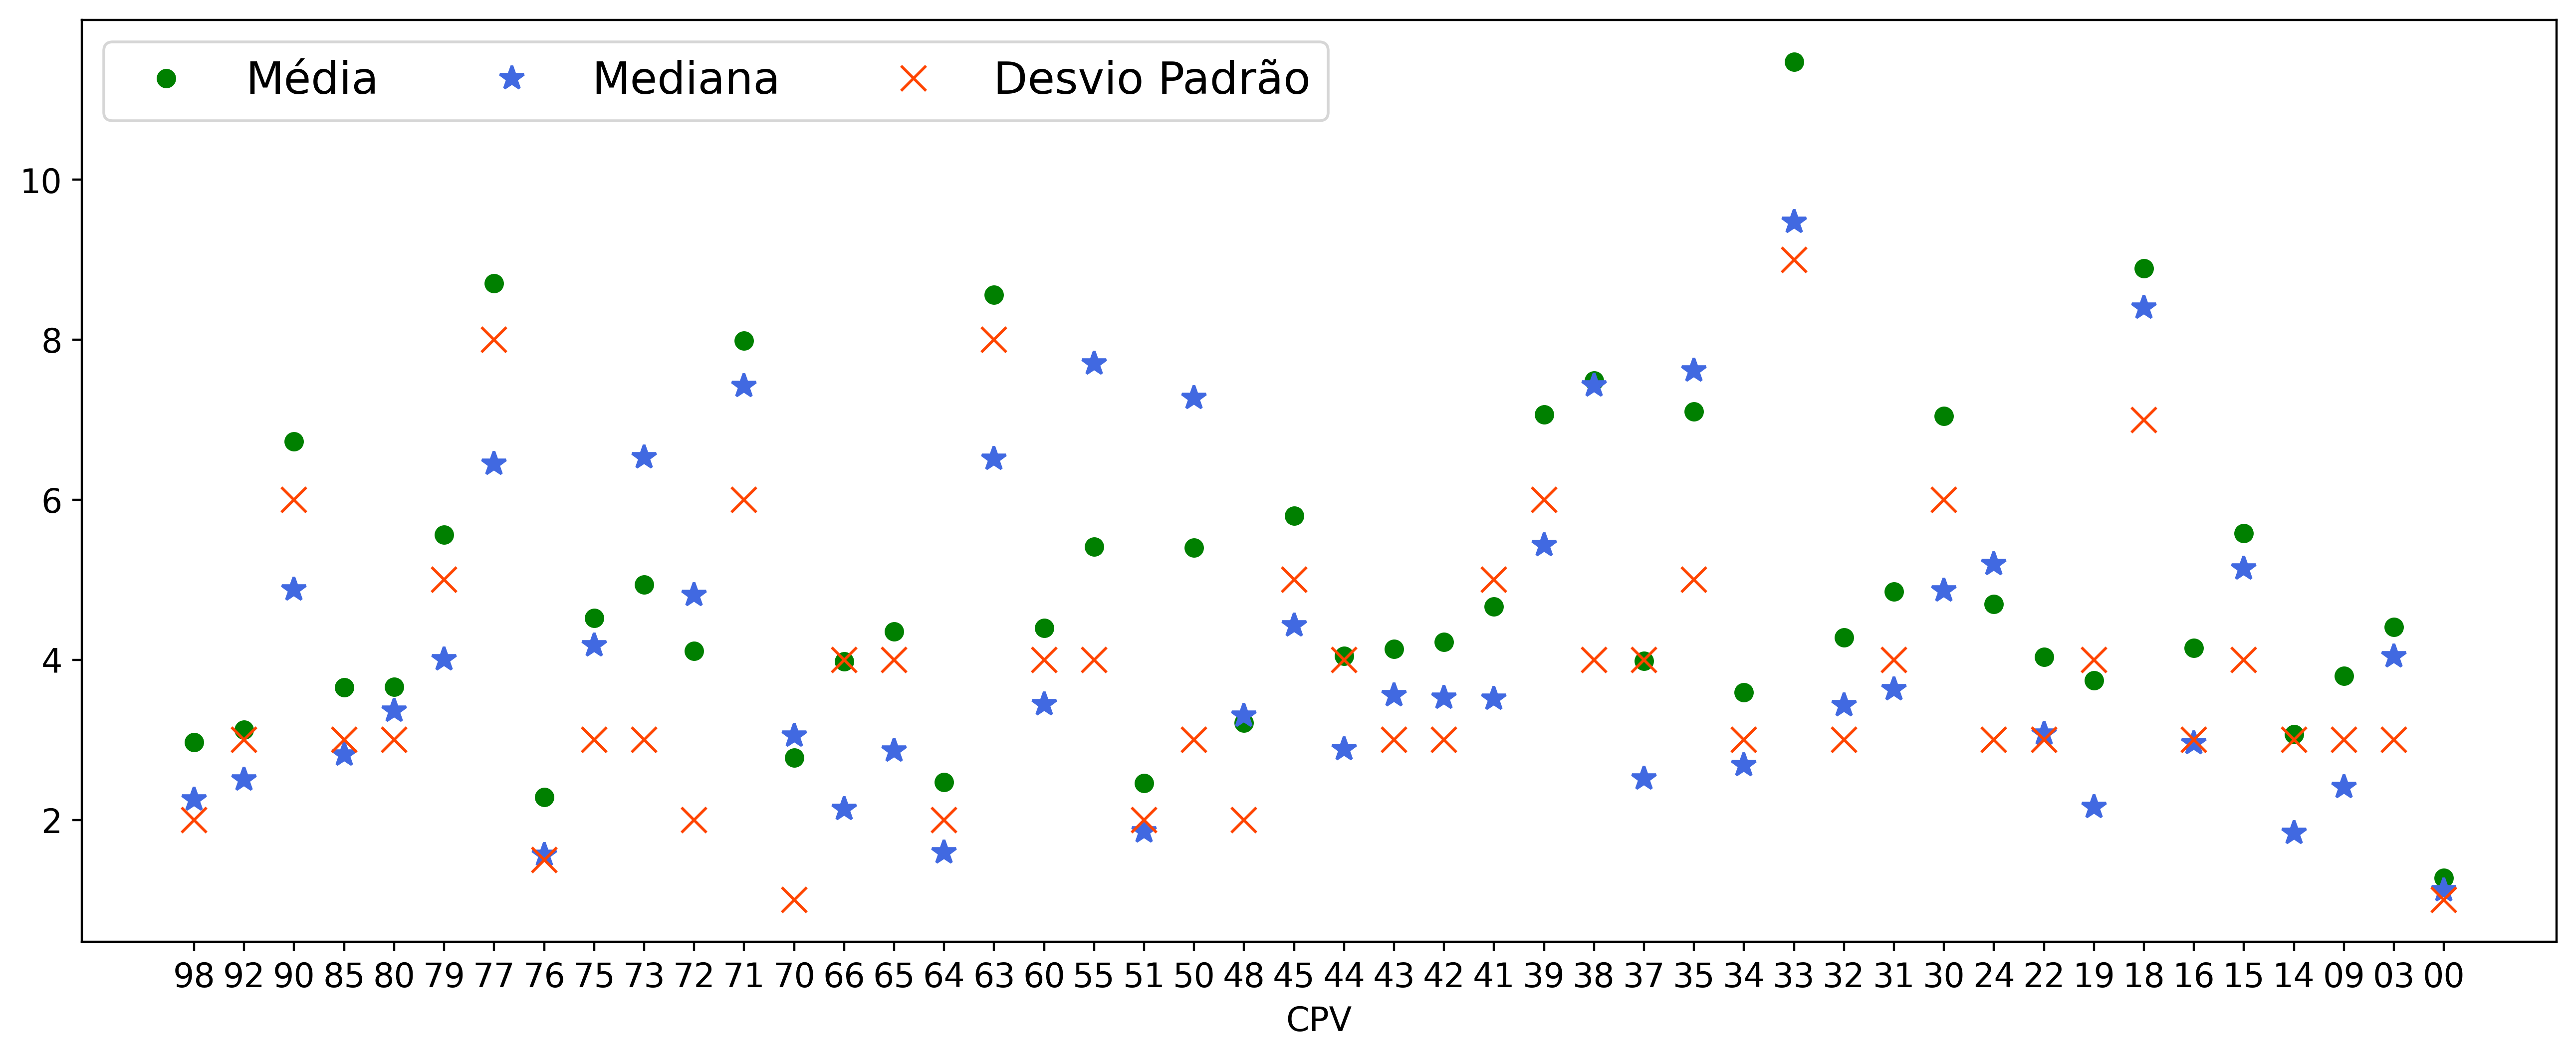
\includegraphics[width=\textwidth]{imagens/mmdp.png}
	\caption{Comparação da Média, Mediana e Desvio Padrão do NEC em CP por CPV}
	\label{}
\end{figure}

Foi, também, feita uma representação gráfica do boxplot para cada umas divisões do CPV. 

%\begin{figure}[!htbp]
%	\centering
%	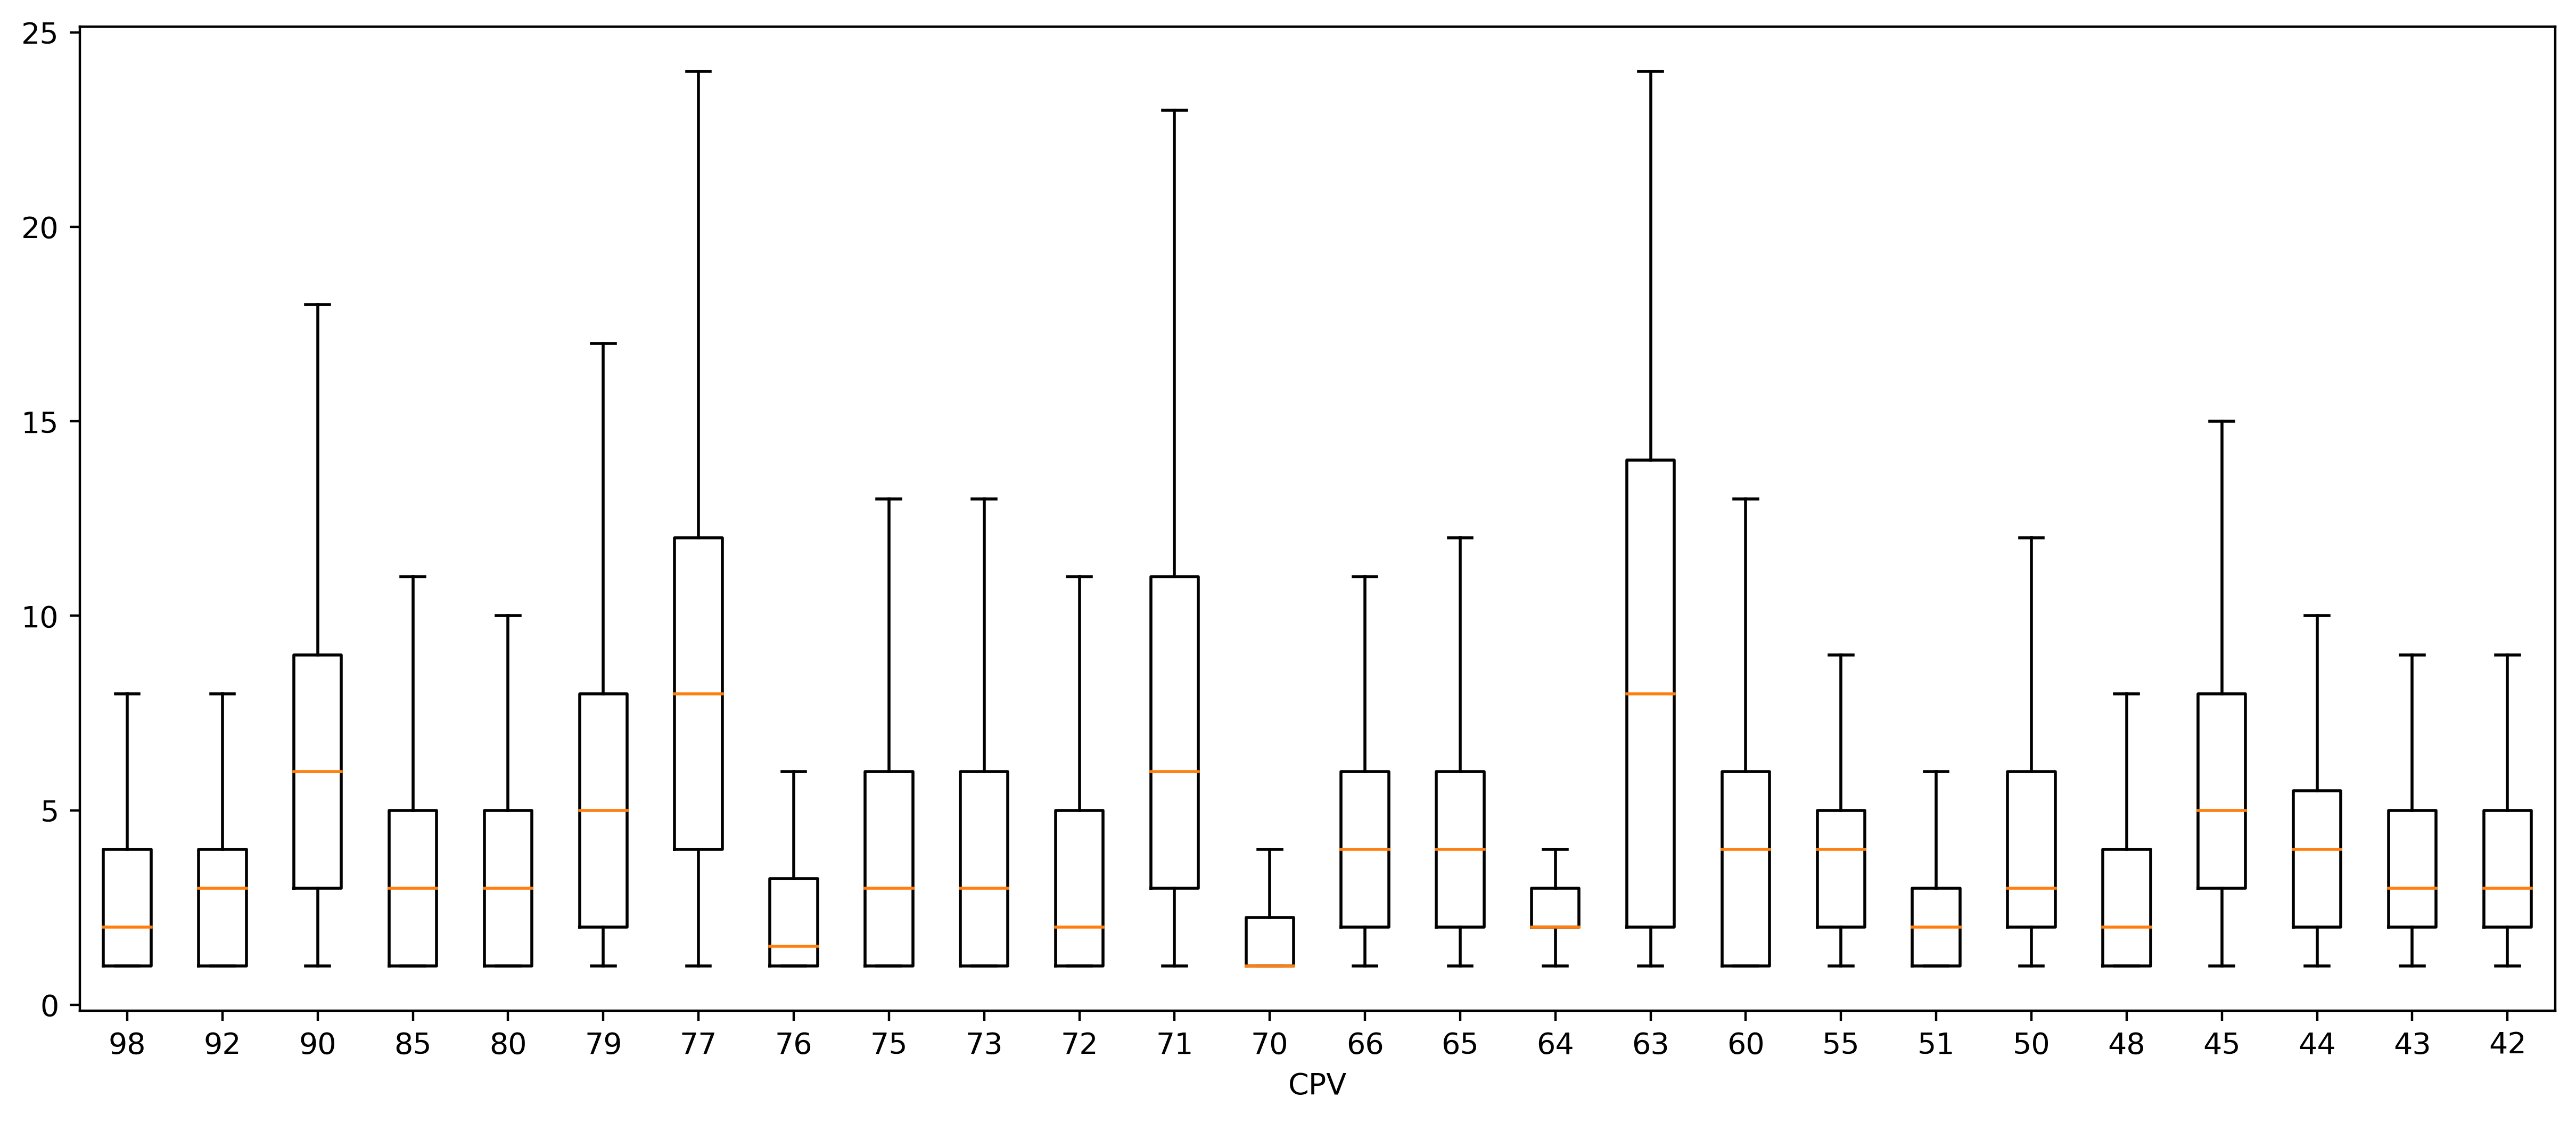
\includegraphics[width=.9\textwidth]{imagens/cpv1.png}
%	\caption{Boxplot referente ao número de entidades concorrentes em Concursos Públicos por CPV : I}
%	\label{}
%\end{figure}
%
%
%\begin{figure}[h!]
%	\centering
%	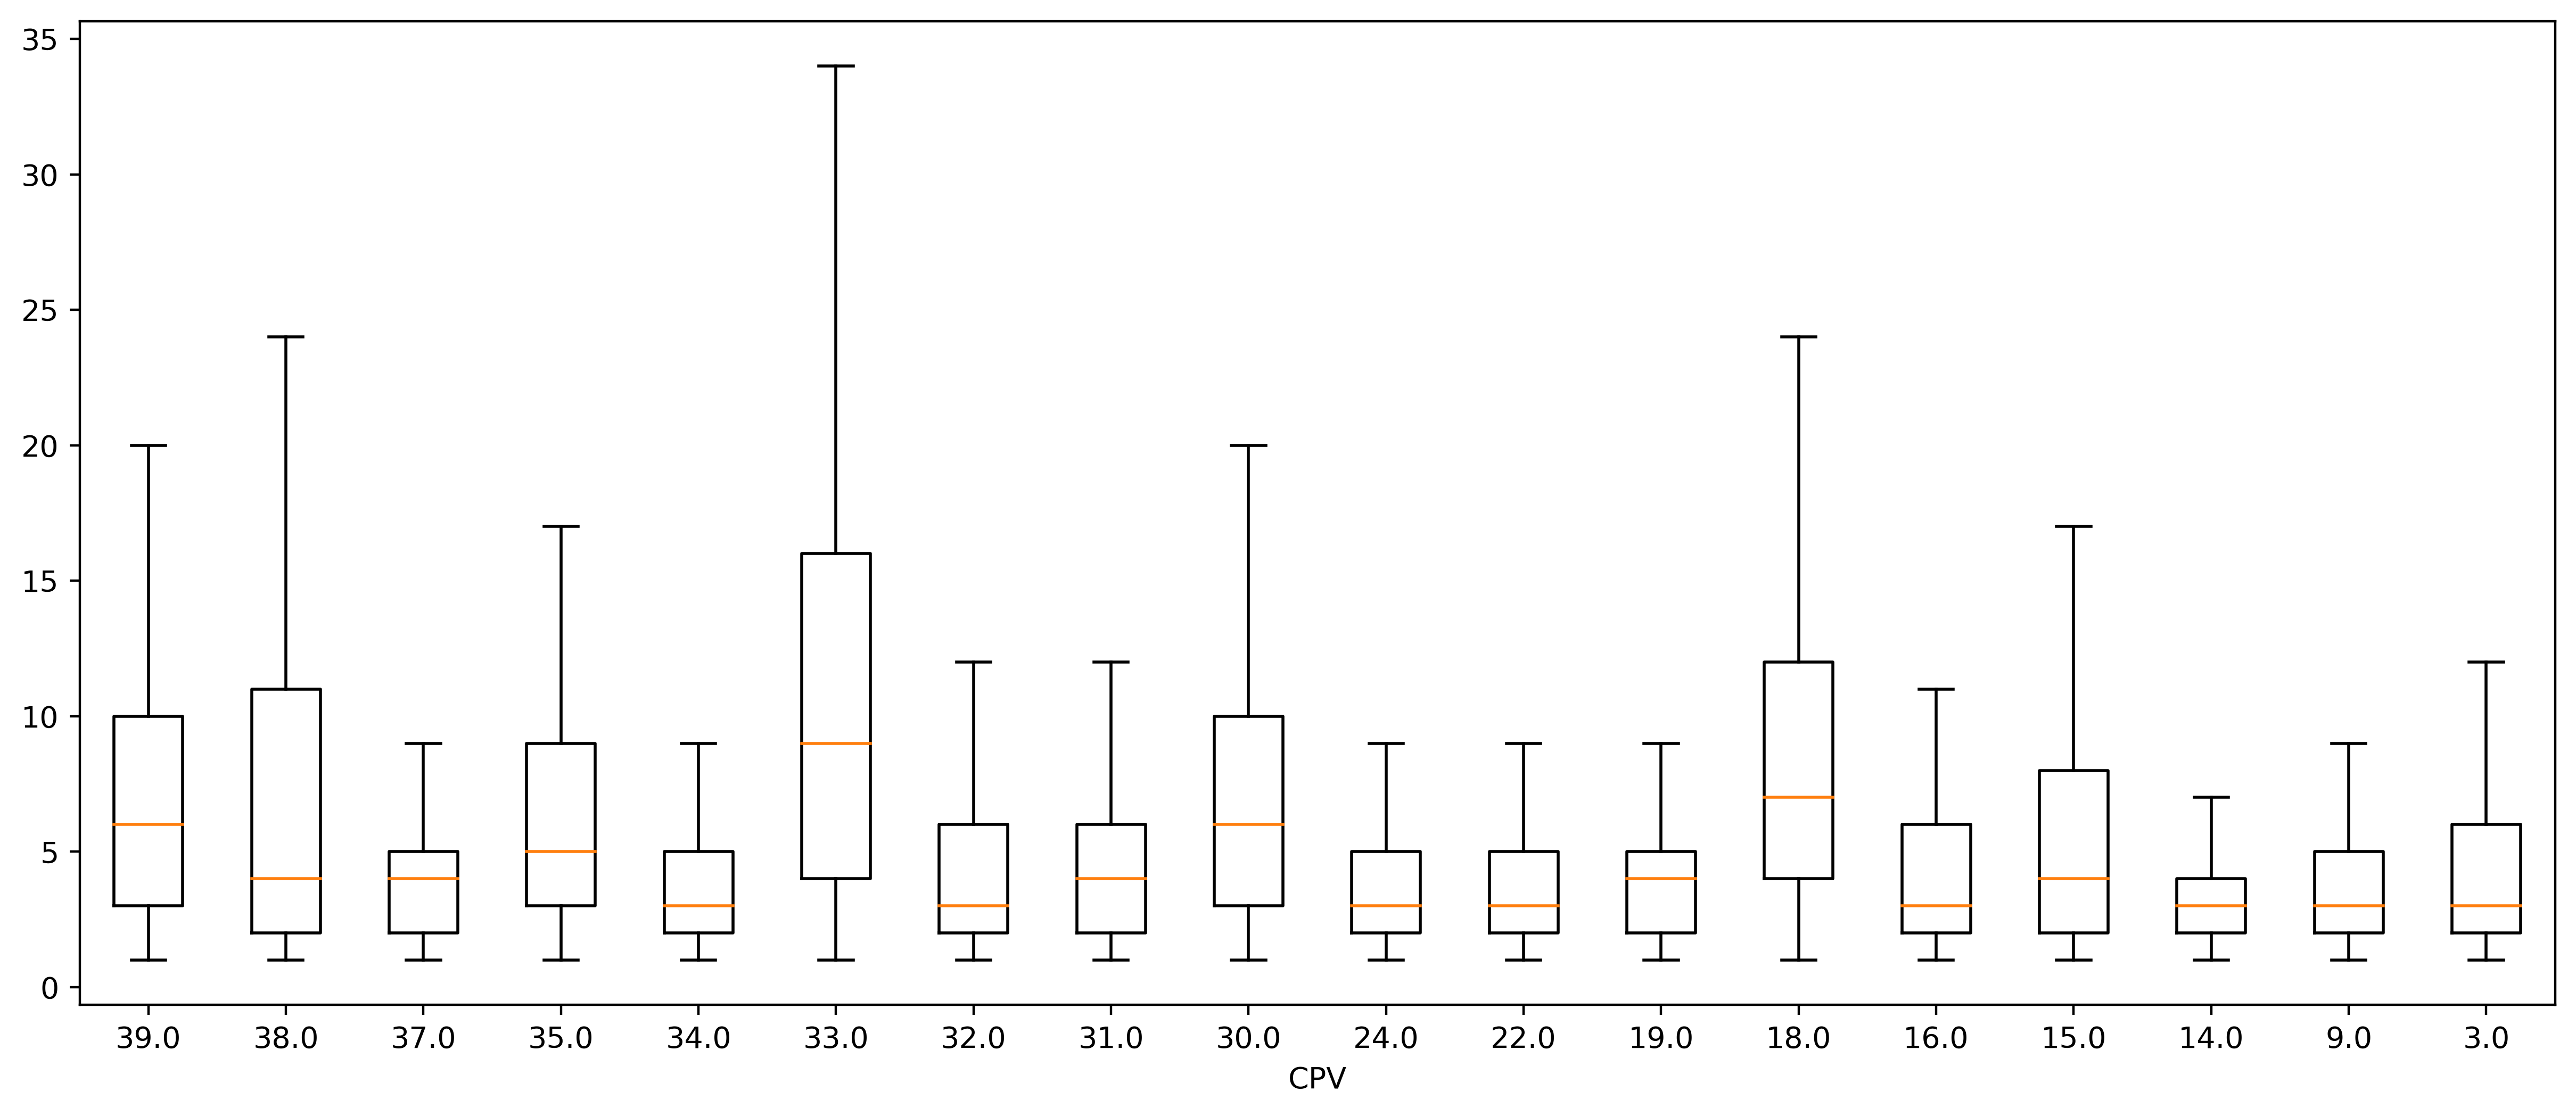
\includegraphics[width=.9\textwidth]{imagens/cpv2.png}
%	\caption{Boxplot referente ao número de entidades concorrentes em Concursos Públicos por CPV : II}
%	\label{}
%\end{figure}

\begin{figure}[H]
	\centering
	\includegraphics[width=.9\textwidth]{imagens/cpv3.png}
	\caption{Boxplot referente ao número de entidades concorrentes em Concursos Públicos por CPV }
	\label{}
\end{figure}


Assim, a fim de selecionarmos os IDs de todos os contratos que respeitem a definição enunciada anteriormente, foi construída a seguinte \textit{query} que retorna todos os contratos cujo número de entidades concorrentes seja inferior à metade do número de entidades concorrentes esperado.  

\begin{lstlisting}[
	language=SQL,
	showspaces=false,
	basicstyle=\ttfamily,
	numbers=left,
	numberstyle=\tiny,
	commentstyle=\color{gray}, frame = single,
	breaklines=true,
	autogobble =true,
	postbreak=\mbox{\textcolor{red}{$\hookrightarrow$}\space},
	]
	SELECT concursospublicos."id"
	FROM concursospublicos 
	JOIN cpv_stat ON concursospublicos."cpv2" = cpv_stat."cpv"
	WHERE concursospublicos."nr_entidadesconcorrentes" < 0.5 * cpv_stat."mean";
\end{lstlisting}

Os resultados obtidos, que podem ser observados na seguinte figura, mostram que existe uma forte predominância dos CPVs começados por 33 e 45, o que pode ser um indicador de que existe um elevado número de contratos com um número \textit{baixo} de entidades concorrentes. 

\begin{figure}[H]
	\centering
	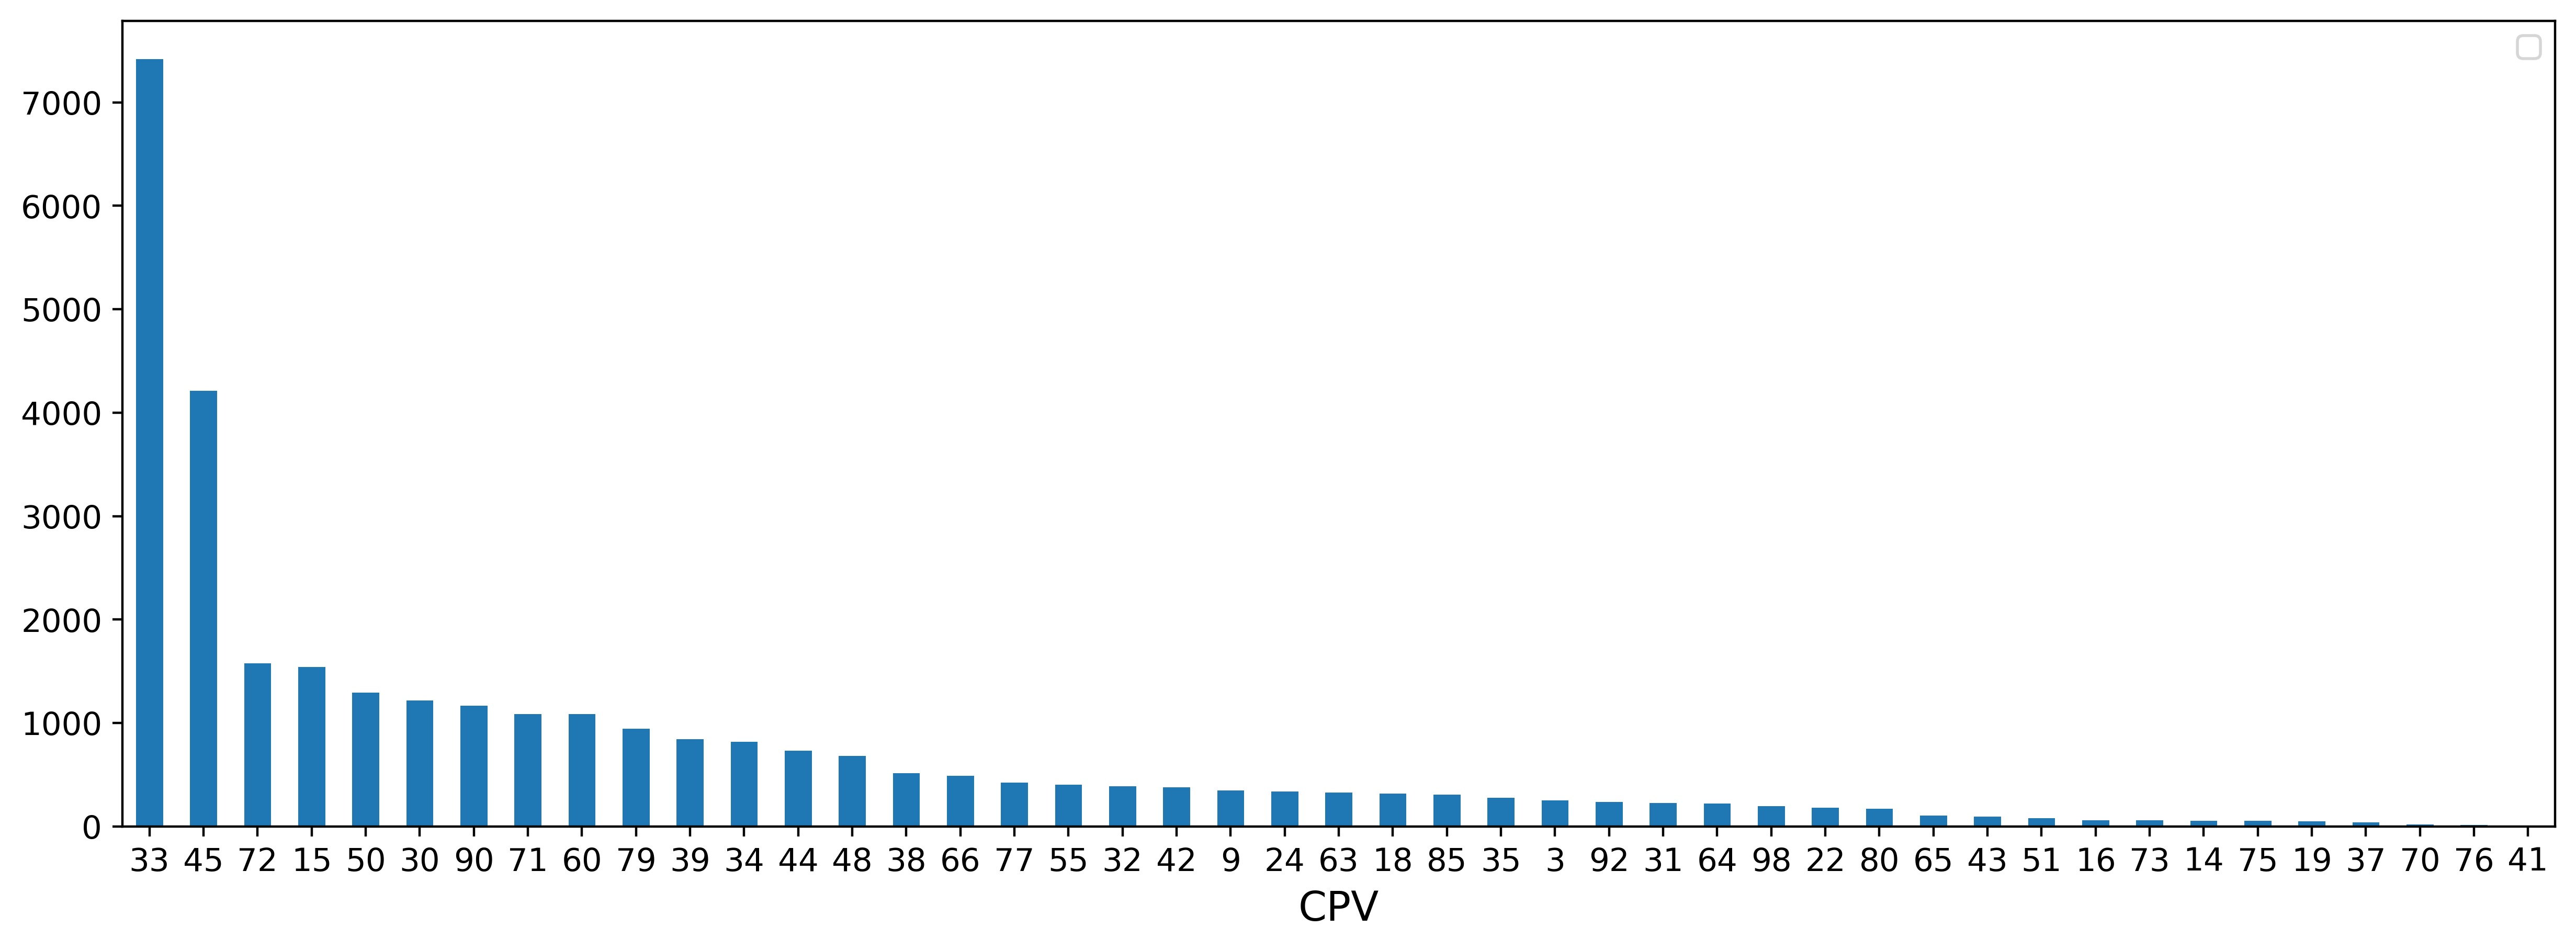
\includegraphics[width=\textwidth]{imagens/r019.png}
	\caption{Grupos com maior número de contratos indiciados}
	\label{}
\end{figure}





\subsection{R031 : Análise da relação entre Preço Base e Preço contratual}

A primeira flag construída tem como objetivo comparar o preço base com o preço contratual.


Numa primeira instância, pegou-se num \textit{subset} de contratos da base de dados em PostgreSQL e guardou-se numa \textit{dataframe} em Python. 
Utilizando a função \textit{cpv}, obtiveram-se os id's dos contratos de um dos tipos de contrato desejados e para um determinado cpv. Numa fase inicial optou-se pelos ids concursos públicos para CPV's começados por 72. 


Para se poder comparar ambos os preços foram desenvolvidas algumas funções auxiliares.
Primeiramente, desenvolveu-se a função \textit{preco\_contratual1} que devolve, a partir do id de um anúncio, o valor do preço contratual desse mesmo anúncio.
A função \textit{preco\_contratual2} faz o mesma coisa mas para um tabela genérica pertencente à base de dados. A função \textit{preco\_contrato3} generaliza a primeira função, pois retorna um conjunto de preços contratuais referentes a um conjunto de ids de anúncios que leva como input. A função \textit{preco\_contratual4} generaliza a função anterior para qualquer tabela. Os precos contratuais são retornados no formato de array.


De seguida, foi feito o mesmo para o preço base. Foi utilizada a mesma abordagem e construíu-se a função \textit{preco\_base3} que retorna os valores dos preços base para um conjunto de id's. 


Assim, foi construída uma primeira versão para esta flag. 

\begin{verbatim}
	def redflag(pbase, pcontr, tol, ids, r, df):
\end{verbatim}

Definiram-se como parâmetros de entrada desta função o conjunto de preços bases - pbase - e preços contratuais - pcontr - associados a um determinado conjunto de ids - ids - que já conseguimos determinar usando as funções criadas anteriormente. É preciso fornecer uma tolerância - tol - que vai definir a diferença máxima permitida entre o preço base e o contratual e um racio máximo permitido entre o preco base e contratual. 


O objetivo desta flag é identificar todos os contratos cujo preço contratual pertença a um intervalo em torno do preço base, definido pelo parâmetro \textit{tol}.

\begin{figure}[H]
	\centering
	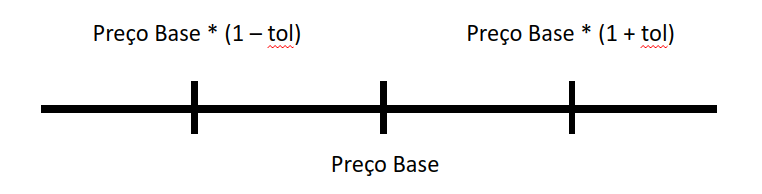
\includegraphics[width=0.7\textwidth]{imagens/pbasecontr.png}
	\caption{}
	\label{}
\end{figure}


%O preço base é conhecido à priori, por isso esta flag não tem muito valor por si só. Quando for acoplada com outras flags pode sugerir um comportamento suspeito. Também é preciso ter em conta como é que o preço base é calculado. Se o preço base for calculado por excesso e o preço contratual for próximo do preço base, pode haver corrupção tanto por parte da entidade adjudicante como da adjudicatária. 

Contudo, ao longo da construção desta flag verificou-se a existência de casos em que o preço base é significativamente superior ao preço contratual, chegando a atingir uma ordem de grandeza de $\approx 10^2$. Isto deve-se a dois fatores : o preço base definido é demasiado elevado comparativamente ao preço contratual ou o preço base diz respeito a casos em que a adjudicação de um determinado serviço/obra é feita por lotes.

\begin{table}[H]
	\centering
	\begin{tabular}{|c|c|c|c|c|}
		\hline
		\multicolumn{1}{|l|}{\textbf{Número de Anúncio}} & \multicolumn{1}{l|}{\textbf{ID}} & \multicolumn{1}{l|}{\textbf{Lote}} & \multicolumn{1}{l|}{\textbf{Preço Base}} & \multicolumn{1}{l|}{\textbf{Preço Contratual}}          \\ \hline
		& 10471090                         & 1                                  &                                          & \cellcolor[HTML]{F2FCFE}{\color[HTML]{555555} 77454.72} \\ \cline{2-3} \cline{5-5} 
		& 10471049                         & 2                                  &                                          & \cellcolor[HTML]{F2FCFE}{\color[HTML]{555555} 85365.84} \\ \cline{2-3} \cline{5-5} 
		\multirow{-3}{*}{11171/2023}                     & 10470972                         & 3                                  & \multirow{-3}{*}{373860.48}              & \cellcolor[HTML]{F2FCFE}{\color[HTML]{555555} 89886.72} \\ \hline
	\end{tabular}
	\caption{Exemplo de contrato adjudicado por lotes}
\end{table}


Tendo em conta que na base de dados não é disponibilizado o preço base para cada lote, foi utilizada a seguinte abordagem. É de salientar que no caso de adjudicação por lotes, o número de anúncio é igual para cada um dos lotes, mas cada lote tem um id diferente. 

Sempre que o rácio $\text{preçobase} / \text{preçocontratual}$, para um certo contrato, é superior a determinado limite, o respetivo id é guardado. A partir do id do contrato obtém-se o número do anúncio e, para todos os contratos com o mesmo número de anúncio, são somados os preços contratuais e o resultado final é comparado com o preço base. 

Por fim, o resultado final é um conjunto de id's na forma de tuplo que respeita as condições anteriormente mencionadas.




%\section{Análise dos Concursos Públicos}
%
%Aqui só foram usadas funções ja definidas. Criaram-se variáveis que guardam o valor do preço base e contratual dos concursos. Deu-se isso como input à funcao \textit{redflag}, além dos outros que são definidos por mim, e obtiveram-se as redflags. Representou-se um barplot dos precos contratuais em cima dos preços base para verificar a diferença entre os mesmos. 


%\section{Análise dos Ajustes Diretos em Regime Geral}
%
%Aqui, novamente, foram utilizadas as funções já criadas anteriormente para obter uma dataframe com os contratos referentes a ajustes diretos e os ids associados. Foi feito um sumário estatístico dos valores dos preços contratuais e um histograma e um boxplot. Mas como tem outliers, vê-se mal. 
%Ordenei os ajustes diretos por fundamentação. Não nenhum campo vazio. 
%Com isto tudo ja se podem calcular as flags usando a função \textit{redflag2}. 
%É interessante saber qual a proporção de atividades suspeitas por entidade adjudicante e entidade adjudicatária. Para isso, calculou-se primeiro o número de contratos suspeitos e respetiva percentagem. 
%Para conseguir analisar foi preciso separar as colunas das entidades adjudicantes e adjudicatárias - que estavam no formato Entidade(NIF)(URL) - em três colunas distintas para cada uma das duas entidades. Isto é necessário para filtrar os contratos pelo NIF porque diferentes entidades podem ter o mesmo NIF. 
%Depois disso, ordenou-se por ordem decrescente de ajustes diretos realizados os NIFS das empresas. Uma das listas ordenadas só para as entidades adjudicantes, outra para as entidades adjudicatárias. 
%Para esta analise foi necessário criar duas funções que retornem os ids dos ajustes diretos a partir do NIF da empresa. Queremos todos os ajustes diretos celebrados para um determinada entidade a partir do seu NIF. Isso foi feito a partir das funções \textit{e\_adjudicante} e \textit{e\_adjudicataria}. 
%De seguida, foi então calculado para cada NIF o número de ajustes diretos realizados usando uma das funções anteriores e os respetivos ID's. Para cada NIF, foi comparado cada um dos nos id's com a lsita de id's dado pela função \textit{redflags2} e feito o rácio para ver a percentagem de contratos suspeitos. 
%Agora seria interessante verificar se existem, dentro destas empresas, subgrupos entre entidades adjudicantes e adjudicatárias. 

\subsection{R051 : Alta concentração de mercado}

\Lemma{}
{A small number of companies concentrate a high share of contracts in a particular market.}



\subsection{RF2 : Comparação entre Preço Contratual e Preço Total Efetivo}

Existem situações em que o valor contratual celebrado é alterado após celebração do contrato, seja por não existir necessidade de usar tantos recursos como a situação oposta. Estes valores são guardados na coluna referefente ao Preço Total Efetivo. Nesses casos, é simples verificar quais são os contratos em que ocorre esta situação através de uma \textit{query}: 

\begin{lstlisting}[
	language=SQL,
	showspaces=false,
	basicstyle=\ttfamily,
	numbers=left,
	numberstyle=\tiny,
	commentstyle=\color{gray},	frame=single,
	breaklines=true,
	autogobble = true,
	postbreak=\mbox{\textcolor{red}{$\hookrightarrow$}\space},
	]
	SELECT contratos_basegov."id", 
		preco_contratual, 
		contratos_basegov."totalEffectivePrice", 
		contratos_basegov."totalEffectivePrice"/preco_contratual AS racio
	FROM contratos_basegov 
	WHERE contratos_basegov."totalEffectivePrice" > 0 AND 
		ABS(contratos_basegov."totalEffectivePrice" - preco_contratual) > 0 AND 
		preco_contratual > 0;
\end{lstlisting}


\begin{figure}[H]
	\centering
	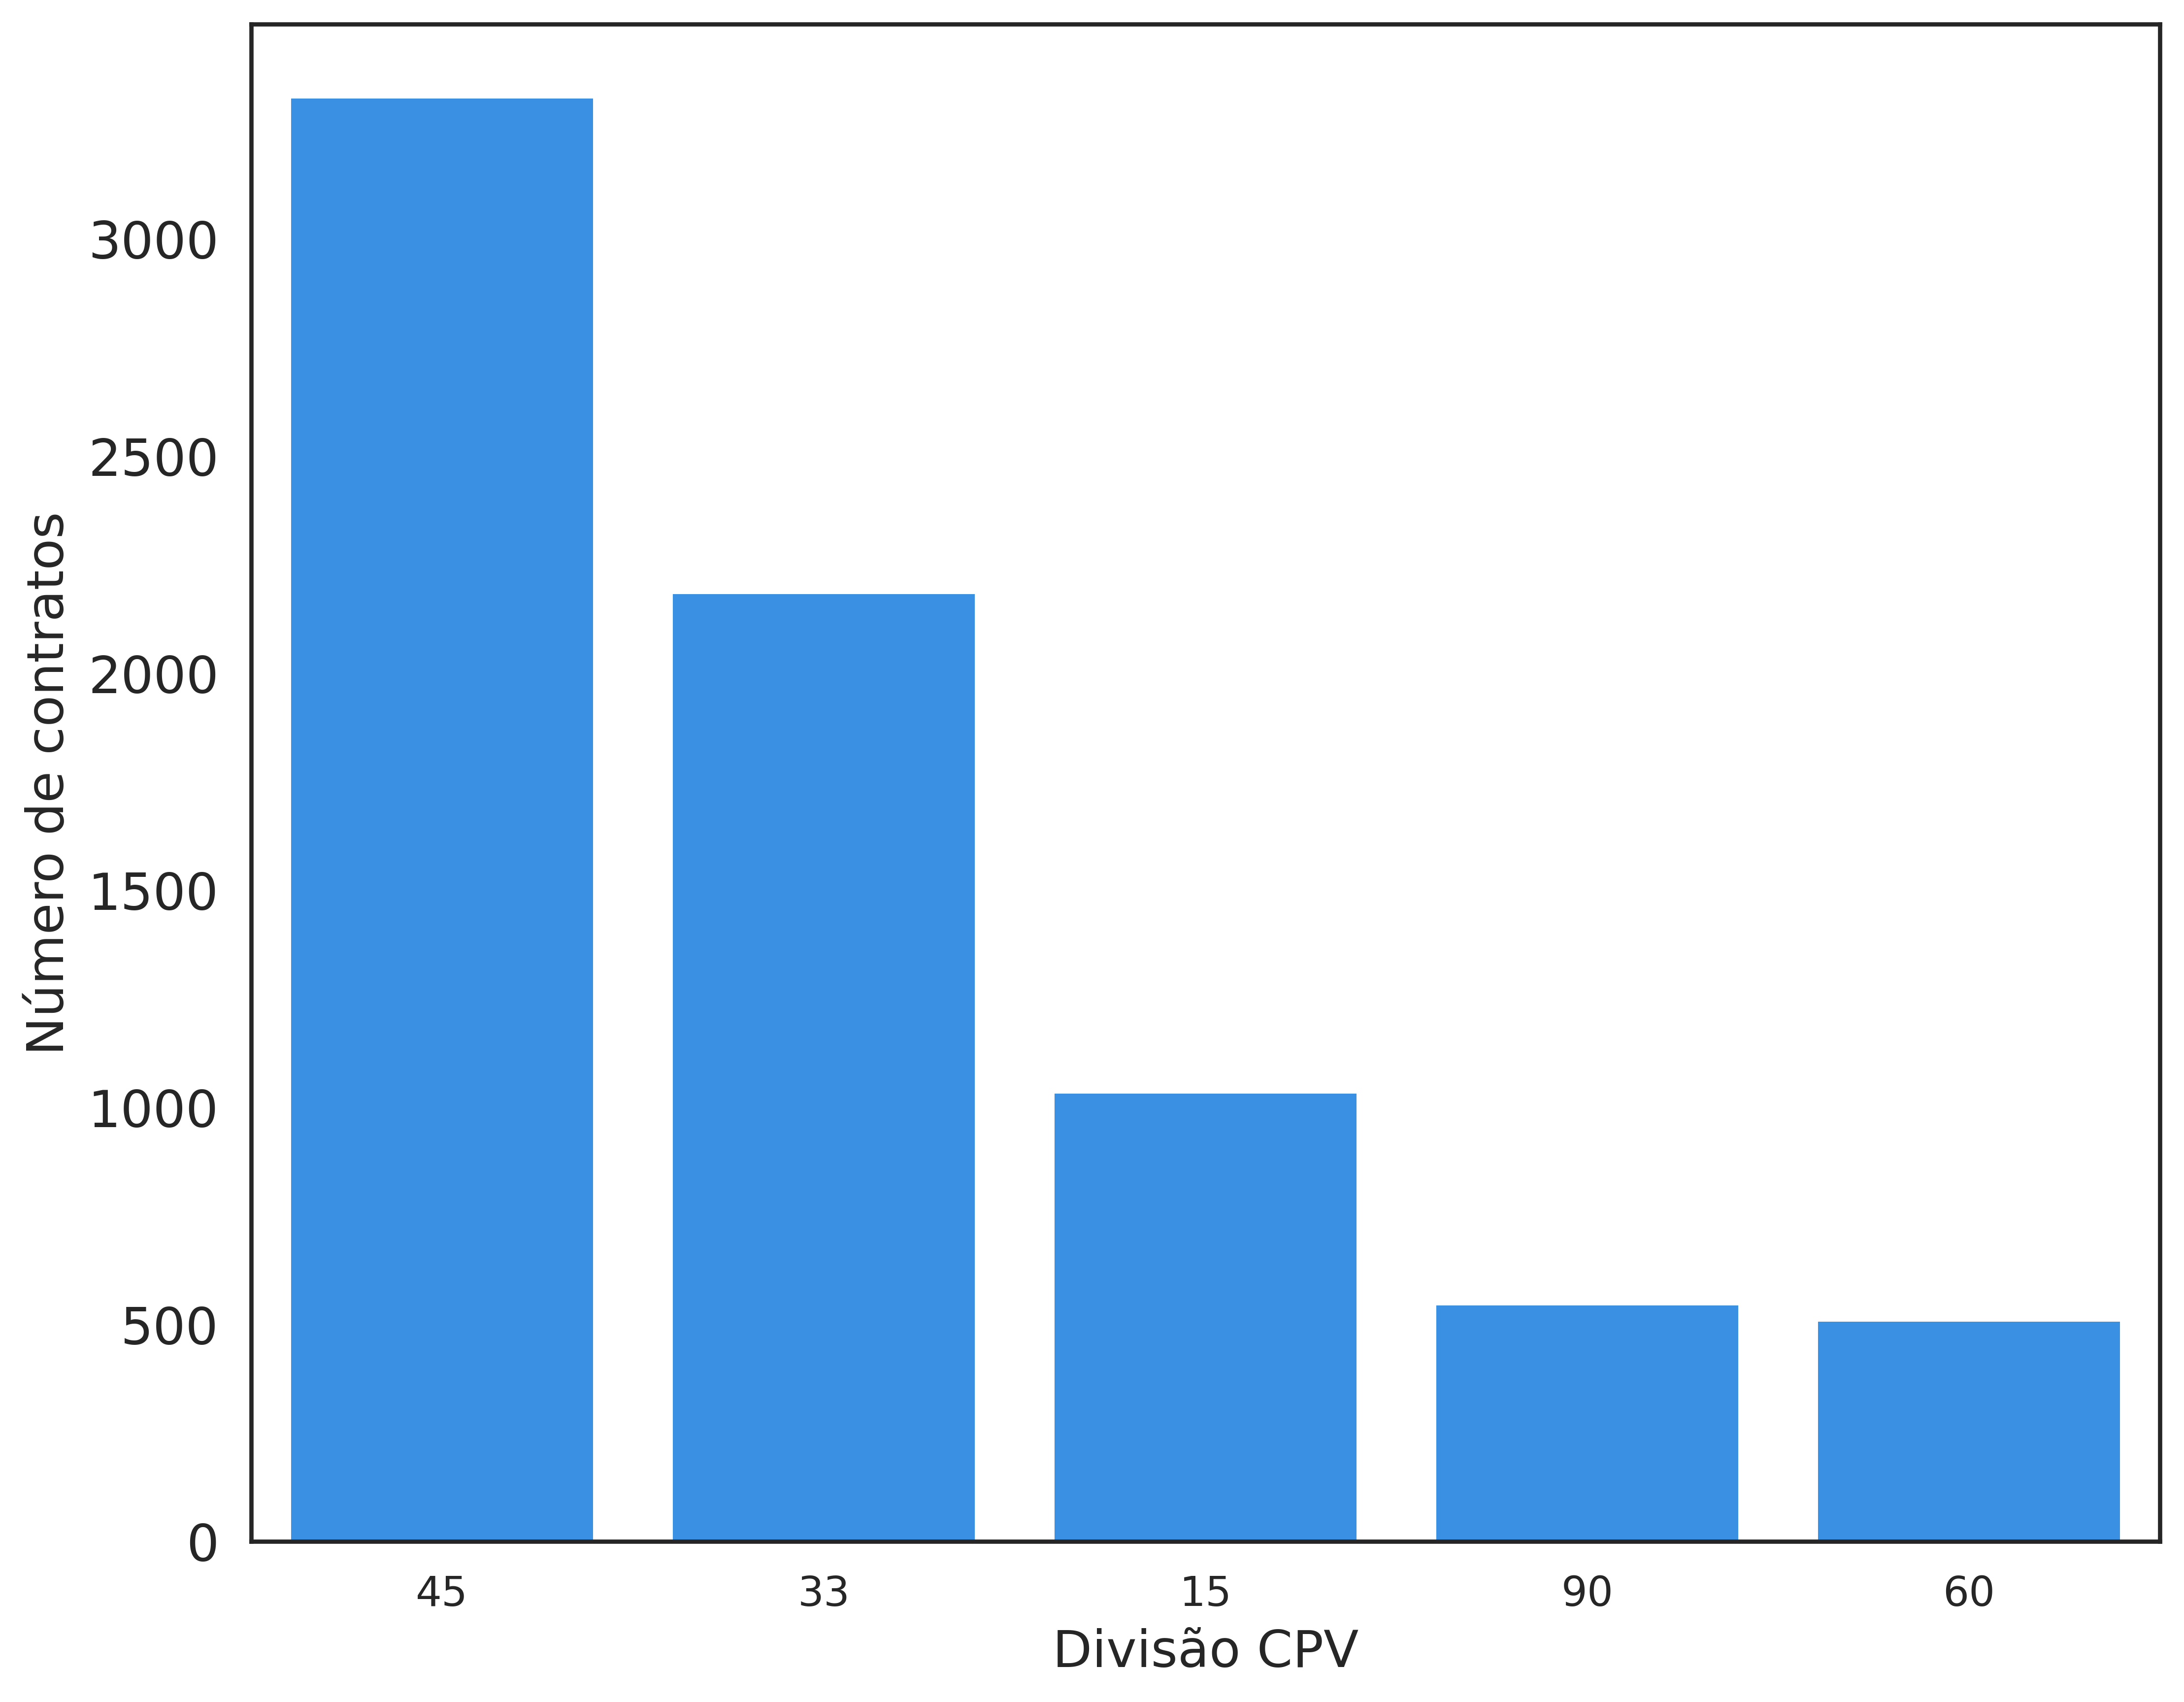
\includegraphics[width=0.5\textwidth]{imagens/rf2/main_cpvs.png}
	\caption{Grupos com maior número de contratos indiciados}
	\label{}
\end{figure}



\subsection{RF3: Análise da data de publicação do anúncio}

Adicionalmente, foi feita uma análise do dia de publicação do anúncio em Diário da República. O objetivo deste indicador é verificar se existem anúncios publicados em dias não convencionais - feriados nacionais - na tentativa de os fazer passar despercebidos. Não existe nenhuma ocorrência deste indicador nos contratos presentes na base de dados durante o período de tempo estudado. 




\section{Processo de Automação}






